	%%%%%%%%%%%%%%%%%%%%%%%%%%%%%%%%%%%%%%%%%%%%%%%%%%%%%%%%%%%%%%%%%%%%%%%%%%%%%%%%
%                         FORMATO DE TESIS FC UNAM                             %
%%%%%%%%%%%%%%%%%%%%%%%%%%%%%%%%%%%%%%%%%%%%%%%%%%%%%%%%%%%%%%%%%%%%%%%%%%%%%%%%
% based on Harish Bhanderi's PhD/MPhil template, then Uni Cambridge
% http://www-h.eng.cam.ac.uk/help/tpl/textprocessing/ThesisStyle/
% corrected and extended in 2007 by Jakob Suckale, then MPI-iCBG PhD programme
% and made available through OpenWetWare.org - the free biology wiki

%                     Under GNU License v3

% ADAPTADO PARA FI-UNAM:  Jesús Velázquez y Marco Ruiz
\sloppy
\documentclass[twoside,11pt]{Latex/Classes/PhDthesisPSnPDF} 
\usepackage{blindtext}
\usepackage[spanish]{babel}
\usepackage{babelbib}
%\usepackage{multicols}
\usepackage{natbib} 
\usepackage{hyperref}
\usepackage{url}
\usepackage{hyperref}
\usepackage{breakurl}
%\usepackage[dvips]{graphicx}
\usepackage{graphicx}
\usepackage{fancyhdr}
\usepackage{multicol}
\usepackage{mathtools}
\usepackage{float}
\usepackage{theorem}
\setlength{\theorempreskipamount}{5mm}
\setlength{\theorempostskipamount}{5mm}
\theoremstyle{break}
\theorembodyfont{\normalfont}
\theoremheaderfont{\scshape}
\newtheorem{thm}{\bf \textit{Teorema} }
\newtheorem{lem}{\bf \textit{Lema}    }
\newtheorem{defini}{\bf \textit{Definición}    }
\newtheorem{corola}{\bf \textit{Corolario}    }
\usepackage{algorithm}
\usepackage{algpseudocode}
\usepackage[all]{xy} %paquete de diagramas
\setcitestyle{square}
\setlength{\parindent}{0cm}
%\usepackage{lipsum}% http://ctan.org/pkg/lipsum
%\usepackage{showframe}% http://ctan.org/pkg/showframe
%\usepackage{eso-pic}% http://ctan.org/pkg/eso-pic
\usepackage{graphicx}% http://ctan.org/pkg/graphicx
\usepackage{tikz}
\usetikzlibrary{shapes.geometric, arrows}
\tikzstyle{startstop} = [rectangle, rounded corners, minimum width=3cm, minimum height=1cm,text centered, draw=black, fill=red!30]
\tikzstyle{io} = [trapezium, trapezium left angle=70, trapezium right angle=110, minimum width=3cm, minimum height=1cm, text centered, draw=black, fill=blue!30]
\tikzstyle{process} = [rectangle, minimum width=3cm, minimum height=1cm, text centered, draw=black, fill=orange!30]
\tikzstyle{decision} = [diamond, minimum width=3cm, minimum height=1cm, text centered, draw=black, fill=green!30]
\tikzstyle{arrow} = [thick,->,>=stealth]
%\usepackage{algorithm2e}
%[ruled,vlined,lined,linesnumbered,algochapter,portugues]

\makeatletter
\def\BState{\State\hskip-\ALG@thistlm}
\makeatother

                     % Para insertar texto dummy, de ejemplo, pues.
% Note:
% The \blindtext or \Blindtext commands throughout this template generate dummy text
% to fill the template out. These commands should all be removed when 
% writing thesis content.
% This file contains macros that can be called up from connected TeX files
% It helps to summarise repeated code, e.g. figure insertion (see below).

%%%%%%%%%%%%%%%%%%%%%%%%%%%%%%%%%%%%%%%%%%%%%%
%            Colores de la UNAM              %
%%%%%%%%%%%%%%%%%%%%%%%%%%%%%%%%%%%%%%%%%%%%%%
%Azul Pantone 541  -->(0,63,119) RGB
\definecolor{Azul}{RGB}{0,63,119}

%Oro Pantone 460  -->(234,221,150) RGB
\definecolor{Oro}{RGB}{234,221,150}


%%%%%%%%%%%%%%%%%%%%%%%%%%%%%%%%%%%%%%%%%%%%%%
%            Comandos para líneas            %
%%%%%%%%%%%%%%%%%%%%%%%%%%%%%%%%%%%%%%%%%%%%%%
%Se define un comando \colorvrule para hacer líneas verticales de color con 3 argumentos: color, ancho, alto
\newcommand{\colorvrule}[3]{
\begingroup\color{#1}\vrule width#2 height#3
\endgroup}

%Se define un comando \colorhrule para hacer líneas horizontales de color con 2 argumentos: color, ancho
\newcommand{\colorhrule}[2]{
\begingroup\color{#1}\hrule height#2
\endgroup}

%%%%%%%%%%%%%%%%%%%%%%%%%%%%%%%%%%%%%%%%%%%%%%
%          Comando para derivadas            %
%%%%%%%%%%%%%%%%%%%%%%%%%%%%%%%%%%%%%%%%%%%%%%
\newcommand{\derivada}[3][]{\ensuremath{\dfrac{\mbox{d}^{#1}#2}{\mbox{d}#3^{#1}}}} 
%primer argumento(opcional): orden de la derivada
%segundo argumento: función a derivar
%tercer argumento: variable respecto a la que se deriva


%%%%%%%%%%%%%%%%%%%%%%%%%%%%%%%%%%%%%%%%%%%%%%
%       Comando para la exponencial          %
%%%%%%%%%%%%%%%%%%%%%%%%%%%%%%%%%%%%%%%%%%%%%%
\newcommand{\e}[1][]{\ensuremath{\mbox{e}^{#1}}}
%primer argumento(opcional): exponente de la exponencial




% insert a centered figure with caption and description
% parameters 1:filename, 2:title, 3:description and label
\newcommand{\figuremacro}[3]{
	\begin{figure}[htbp]
		\centering
		\includegraphics[width=1\textwidth]{cabezaaa}
		\caption[#2]{\textbf{#2} - #3}
		\label{condicion}
	\end{figure}
}

% insert a centered figure with caption and description AND WIDTH
% parameters 1:filename, 2:title, 3:description and label, 4: textwidth
% textwidth 1 means as text, 0.5 means half the width of the text
\newcommand{\figuremacroW}[4]{
	\begin{figure}[htbp]
		\centering
		\includegraphics[width=#4\textwidth]{#1}
		\caption[#2]{\textbf{#2} - #3}
		\label{#1}
	\end{figure}
}

% inserts a figure with wrapped around text; only suitable for NARROW figs
% o is for outside on a double paged document; others: l, r, i(inside)
% text and figure will each be half of the document width
% note: long captions often crash with adjacent content; take care
% in general: above 2 macro produce more reliable layout
\newcommand{\figuremacroN}[3]{
	\begin{wrapfigure}{o}{0.5\textwidth}
		\centering
		\includegraphics[width=0.7\textwidth]{#1}
		\caption[#2]{{\small\textbf{#2} - #3}}
		\label{#1}
	\end{wrapfigure}
}

% predefined commands by Harish
\newcommand{\PdfPsText}[2]{
  \ifpdf
     #1
  \else
     #2
  \fi
}

\newcommand{\IncludeGraphicsH}[3]{
  \PdfPsText{\includegraphics[height=#2]{#1}}{\includegraphics[bb = #3, height=#2]{#1}}
}

\newcommand{\IncludeGraphicsW}[3]{
  \PdfPsText{\includegraphics[width=#2]{#1}}{\includegraphics[bb = #3, width=#2]{#1}}
}

\newcommand{\InsertFig}[3]{
  \begin{figure}[!htbp]
    \begin{center}
      \leavevmode
      #1
      \caption{#2}
      \label{#3}
    \end{center}
  \end{figure}
}






%%% Local Variables:
%%% mode: latex
%%% TeX-master: "~/Documents/LaTeX/CUEDThesisPSnPDF/thesis"
%%% End:
           % Archivo con funciones útiles
%%%%%%%%%%%%%%%%%%%%%%%%%%%%%%%%%%%%%%%%%%%%%%%%%%%%%%%%%%%%%%%%%%%%%%%%%%%%%%%%
%                                   DATOS                                      %
%%%%%%%%%%%%%%%%%%%%%%%%%%%%%%%%%%%%%%%%%%%%%%%%%%%%%%%%%%%%%%%%%%%%%%%%%%%%%%%%
\title{C\'alculo de variedades invariantes en \'orbitas peri\'odicas.}
\LARGE\author{Evelyn Álvarez Cruz}        
\degree{Maestra en Maten\'aticas}               % Carrera
\director{Dr. Renato Carlos Calleja}               % Director de tesis
\degreedate{2021}                           % Año de la fecha del examen
\lugar{Ciudad Universitaria, CD.MX. }                        % Lugar
%\portadafalse                              % Portada en NEGRO, descomentar y comentar la línea siguiente si se quiere utilizar
\portadatrue                                % Portada en COLOR

\keywords{tesis,autor,tutor,etc}            % Palablas clave para los metadatos del PDF
\subject{tema_1,tema_2}    

           % Tema para metadatos del PDF  

%%%%%%%%%%%%%%%%%%%%%%%%%%%%%%%%%%%%%%%%%%%%%%%%%%%%%
%                   PORTADA                         %
%%%%%%%%%%%%%%%%%%%%%%%%%%%%%%%%%%%%%%%%%%%%%%%%%%%%%
\begin{document}
\maketitle									% Se redefinió este comando en el archivo de la clase para generar automáticamente la portada a partir de los datos

%%%%%%%%%%%%%%%%%%%%%%%%%%%%%%%%%%%%%%%%%%%%%%%%%%%%%
%                  PRÓLOGO                          %
%%%%%%%%%%%%%%%%%%%%%%%%%%%%%%%%%%%%%%%%%%%%%%%%%%%%%
\frontmatter
%%\chapter*{}
%\pagenumbering{Roman}

\begin{tabular}{ll}
\textbf{1. Datos de la alumna}	&  \\ 
Apellido paterno:	& Álvarez  \\ 
Apellido materno:	& Cruz \\ 
Nombre(s):	& Evelyn \\ 
Teléfono:	& 5521664066 \\ 
Universidad	:& Universidad Nacional Autónoma de México  \\ 
Facultad:	& Facultad de Ciencias  \\ 
Carrera:	& Física \\ 
Número de cuenta:	& 309112426 \\ 
	&  \\ 
\textbf{2. Datos del tutor	}&  \\ 
Grado:	&  Dr.\\ 
Nombre(s):	&  Luis\\ 
Apellido paterno	& Benet \\ 
Apellido materno	&  Fernández\\ 
	&  \\ 
\textbf{3. Datos del sinodal 1	}&  \\ 
Grado:	&  Dr.\\ 
Nombre(s):	&  David\\ 
Apellido paterno	& Philip\\ 
Apellido materno	&  Sanders\\ 
	&  \\ 
\textbf{4. Datos del sinodal 2	}&  \\ 
Grado:	&  Dr.\\ 
Nombre(s):	&  Christof Friedrich\\ 
Apellido paterno	& Jung\\ 
Apellido materno	&  Kohl\\ 
&  \\
\textbf{3. Datos del sinodal 3	}&  \\ 
Grado:	&  Dr.\\ 
Nombre(s):	&  Renato Carlos\\ 
Apellido paterno	& Calleja\\ 
Apellido materno	&  Castillo\\ 
&  \\  
\textbf{3. Datos del sinodal 4	}&  \\ 
Grado:	&  Dr.\\ 
Nombre(s):	&  Ricardo Atahualpa\\ 
Apellido paterno	& Solórzano\\ 
Apellido materno	&  Kraemer\\ 
&  \\  	
\textbf{Datos del trabajo escrito}& \\
Título:& Método de parametrización: Variedades estables e inestables \\
& en mapeos Hamiltonianos de dos dimensiones.\\
Número de páginas:& 61\\
Año:&2019\\
\end{tabular} \\

















%\begin{dedication}
A mi familia. \\



\end{dedication}
 
% ******************************* Thesis Declaration ********************************

\begin{declaration}

Por la presente declaro que, salvo cuando se haga referencia específica al trabajo de otras personas, el contenido de esta tesina es original y no se ha presentado total o parcialmente para su consideración para cualquier otro título o grado en esta o cualquier otra Universidad. Esta tesina es resultado de mi propio trabajo y no incluye nada que sea el resultado de algún trabajo realizado en colaboración, salvo que se indique específicamente en el texto. 
% Author and date will be inserted automatically from thesis.tex

\end{declaration}
  
%%\chapter*{}
%\pagenumbering{Roman}

\begin{acknowledgements}
Gracias a:\\

El Dr. Luis Benet Fernández, quién me guió en la elaboración de esta tesis. Por su tiempo, paciencia y experiencia, que me ayudaron a completar mi educación como universitaria. Por contagiarme de nuevo el entusiasmo por la ciencia en general, la pasión por la física y la enseñanza de la misma. \\

Al  Dr. Christof Jung, al Dr. David P. Sanders, al Dr. Renato Calleja y al Dr. Ricardo A. Solórzano, que con sus valiosos comentarios nutrieron el contenido de este trabajo. Algunas de las secciones se crearon a partir de sus preguntas o sugerencias. \\

Al Dr. Marcos Ley Koo quién me mostró una cara de la física que no se aprende en las aulas, esa que se descubre en todos lados y que te hace un físico fuera de la academia. Que con sus pláticas me llenaba la mente de preguntas que muchas veces me quitaron el sueño. Quién siempre me sorprendía con una nueva forma de entender la termodinámica, a partir de la mecánica o del electromagnetismo y hasta de la geometría. Por compartir sus locas ideas conmigo. \\

A mi familia, sobre todo a mis padres, que con su esfuerzo, valentía y trabajo lograron que cumpliera con mis estudios universitarios. Por la educación que me dieron, con la que aprendí a disfrutar las cosas más simplemente bellas y con la que me he guiado hasta este momento. Por enseñarme a ser crítica, buscar, preguntar y observar, mostrándome que todo eso no se obtiene de un título universitario y tampoco va acompañado de traje, que se puede encontrar en un conductor de tráiler o en un comerciante. A mis hermanos por ser mi apoyo constante, mis compañeros eternos y mis cómplices.\\

A \textquotedblleft el lugar\textquotedblright, a mis amigos, los que están cerca o al otro lado del mundo, por compartir conmigo la vida escolar, por hacerla divertida y memorable. Por intercalar horas de estudio con interminables charlas, risas, con juegos de mesa de 6 horas o con domingos de series.\\

A quién vio esta tesis desde que apenas tenía el nombre y que estuvo presente en todo el proceso, quién me escuchó maldecir cuando el código no funcionaba y me vio pelear con el módulo de álgebra lineal muchas noches. Por ser mi confidente y enseñarme que \textquotedblleft una pasión es una pasión\textquotedblright.\\

Finalmente, al Programa de Apoyo a Proyectos de Investigación e Innovación Tecnológica(PAPIIT) de la Dirección General de Asuntos del Personal Académico (DGAPA) de la UNAM con clave IG100616, por la beca recibida.

\end{acknowledgements}




     % Comentar línea si no se usa

\chapter{Introducción}

El estudio de órbitas perri\'odicas hiperb\'olicas es un tema interesante en el estudio de los sistemas din\'amicos discretos. En particular el estudio de los conjuntos invariantes asociados a tales \'orbitas es un tema de inter\'es para quienes estudian la teor\'ia KAM (Kolmogorov–Arnold–Moser). Uno de los problemas abiertos en sistemas din\'amicos es el estudio del rompimiento de toros invariantes para mapeos simpl\'ecticos. Tal problema puede ser abordado desde el estudio del comportamiento de las variedades estables e inestables de \'orbitas hiperb\'olicas. \\

En este trabajo se presenta la implementaci\'on de un m\'etodo para encontrar \'orbitas peri\'odicas de mapeos simpl\'ecticos de dos dimensiones y para parametrizar las variedades asociadas a aquellas \'orbitas que resulten ser hiperb\'olicas. El objetivo es dar una herramienta para el estudio del rompimiento de los toros invariantes. 

            % ~10 páginas - Explicar el propósito de la tesis
  % Comentar línea si no se usa 
%% ******************************* Thesis Declaration ********************************

\begin{declaration}

Por la presente declaro que, salvo cuando se haga referencia específica al trabajo de otras personas, el contenido de esta tesina es original y no se ha presentado total o parcialmente para su consideración para cualquier otro título o grado en esta o cualquier otra Universidad. Esta tesina es resultado de mi propio trabajo y no incluye nada que sea el resultado de algún trabajo realizado en colaboración, salvo que se indique específicamente en el texto. 
% Author and date will be inserted automatically from thesis.tex

\end{declaration}
           % Comentar línea si no se usa
%\include{Resumen/Resumen}                   % Comentar línea si no se usa

%%%%%%%%%%%%%%%%%%%%%%%%%%%%%%%%%%%%%%%%%%%%%%%%%%%%%
%Esta sección genera el índice
\setcounter{secnumdepth}{3} % organisational level that receives a numbers%                   ÍNDICES                         %
%%%%%%%%%%%%%%%%%%%%%%%%%%%%%%%%%%%%%%%%%%%%%%%%%%%%%
\setcounter{tocdepth}{3}    % print table of contents for level 3
\tableofcontents            % Genera el índice 
%: ----------------------- list of figures/tables ------------------------
%\listoffigures              % Genera el ínidce de figuras, comentar línea si no se usa
%\listoftables               % Genera índice de tablas, comentar línea si no se usa


%%%%%%%%%%%%%%%%%%%%%%%%%%%%%%%%%%%%%%%%%%%%%%%%%%%%%
%                   CONTENIDO                       %
%%%%%%%%%%%%%%%%%%%%%%%%%%%%%%%%%%%%%%%%%%%%%%%%%%%%%
% the main text starts here with the introduction, 1st chapter,...
\mainmatter
\def\baselinestretch{1.5}                   % Interlineado de 1.5
%%%%%%%%%%%%%%%%%%%%%%%%%%%%%%%%%%%%%%%%%%%%%%%%%%%%%%%%%%%%%%%%%%%%%%%%%
%           Capítulo 2: MARCO TEÓRICO - REVISIÓN DE LITERATURA
%%%%%%%%%%%%%%%%%%%%%%%%%%%%%%%%%%%%%%%%%%%%%%%%%%%%%%%%%%%%%%%%%%%%%%%%%

\chapter{Teor\'ia}
Consideremos un mapeo $M$ que preserva \'area, donde $M:\mathbb{S} \times \mathbb{R} \longrightarrow \mathbb{S}\times\mathbb{R}$. El mapeo $M$ lleva puntos $v_{i}= (x_{i},y_{i})$ en puntos dados por $M(v_{i})=v_{i+1}$, donde el sub\'indice denota que se trata de la i-\'esima iteraci\'on. \\

Nos interesa centrarnos en los mapeos que violan la condici\'on de no degeneraci\'on tambi\'en llamada \textit{condici\'on twist} \cite{Olvera} que dice que 
\begin{eqnarray}
\frac{\partial x_{i+1}}{\partial y_{i}} \neq 0.
\label{twist condition}
\end{eqnarray}
Un mapeo puede violar la condici\'on \ref{twist condition} de diferentes maneras, en especial si para alg\'un valor particular de $y_{i}$ ocurre que $\partial x_{i+1}/\partial y_{i} = 0$. La violaci\'on de la condici\'on \ref{twist condition} da lugar a bifurcaciones de los c\'irculos invariantes, las cuales a su vez son indicadoras de una colisi\'on de \'orbitas peri\'odicas en el mapeo. El valor del par\'ametro para el cual ocurre la colisi\'on es de importancia en teor\'ia KAM. 

\section{Un m\'etodo para encontrar \'orbitas peri\'odicas de mapeos de 2D.}

Los m\'etodos para encontrar \'orbitas peri\'odicas en mapeos de dos dimensiones son generalmente m\'etodos para encontrar ra\'ices de sistemas no lineales en dos dimensiones. En este caso se busca reducir la dimensi\'on en la que se trabaja para encontrar \'orbitas peri\'odicas. Para ello es necesario encontrar algunas simetr\'ias que reduzcan el problema a una dimensi\'on. Veremos que las \'orbitas peri\'odicas se pueden encontrar usando simetr\'ias e involuciones. \cite{GreeneA}\\

Decimos que el mapeo $M$ permanece invariante bajo un mapeo $T$ o que conmuta con $T$ si 
\begin{eqnarray}
TM = MT,
\label{conmuta}
\end{eqnarray}
esta caracter\'istica nos ayudar\'a a redefinir una \'orbita peri\'odica del mapeo. Por otro lado decimos que una transformaci\'on $I$ se dice de \textit{tiempo inverso} para $M$ si 
\begin{eqnarray}
I_{0}M^{-1} = MI_{0}.
\label{involucion1}
\end{eqnarray}
Es decir si la simetr\'ia cambia el sentido del mapeo hacia atr\'as. Si adem\'as la simetr\'ia de tiempo inverso es una involuci\'on ($I_{0}^{2}=1$) se puede construir una nueva involuci\'on a partir de la anterior mediante 
\begin{equation}
I_{1} = MI_{0}.
\label{involucion2}
\end{equation}
Es simple comprobar que $I_{1}$ es involuci\'on, usando la definici\'on \ref{involucion1} tenemos que 
\begin{equation*}
I_{1}^{-1}MI_{1} = (MI_{0})^{-1}MI_{1} = I_{0}^{-1}M^{-1}MI_{1} = I_{0}^{-1}I_{1} = I^{-1}_{0}MI_{0}=M^{-1},
\end{equation*}
y reacomodando t\'erminos obtenemos $I_{0}M^{-1}= MI_{0}$.\\

 
Con las involuciones definidas arriba podemos escribir el mapeo $M$ como factorizaci\'on de las mismas \cite{Devaney3}
\begin{eqnarray}
M = I_{1}I_{0}.
\end{eqnarray}
Decimos entonces que el mapeo $M$ es reversible. Usando estos conceptos vamos a analizar la siguiente afirmaci\'on. \\

\begin{thm}
Sea $M:\mathbb{S} \times \mathbb{R} \longrightarrow \mathbb{S}\times\mathbb{R}$ un mapeo simpl\'ectico no-twist reversible. Sean 
\begin{eqnarray}
\mathbb{J}_{0} = \{v \in \mathbb{S} \times \mathbb{R} | I_{0}v = v\}
\end{eqnarray}
\begin{eqnarray}
\mathbb{J}_{1} = \{v \in \mathbb{S} \times \mathbb{R} | I_{1}v = v\}
\end{eqnarray}
Si $v_{0}\in \mathbb{J}_{0}$ y $M^{N}v_{0}=v_{N}\in \mathbb{J}_{0}$ entonces $v_{0}$ es de periodo $2N$.
\end{thm}
\textit{Demostraci\'on:}\\
Queremos probar que $M^{2N}v_{0}=v_{0}$. Entonces
\begin{align*}
	M^{2N}v_{0} &= M^{N}M^{N}v_{0}\\
				&= M^{N-1}MM^{N-1}Mv_{0}\\
				&= M^{N-1}MM^{N-1}I_{1}I_{0}v_{0},
\end{align*}
usando que $v_{0}\in I_{0}$ y que $M$ es reversible
\begin{align*}
	M^{2N}v_{0} &= M^{N-1}I_{1}I_{0}M^{N-1}I_{1}v_{0},
\end{align*}
usando que $M^{N}v_{0}=v_{N}\in \mathbb{J}_{0}$ y que $M^{N-1}=M^{N}M^{-1}$
\begin{align*}
	M^{2N}v_{0} &= M^{N-1}I_{1}I_{0}M^{N}M^{-1}I_{1}v_{0}\\
				&= M^{N-1}I_{1}	M^{N-1}I_{1}v_{0}.
\end{align*}
Usando que el mapeo es reversible es f\'acil ver que se cumple que
\begin{equation}
I_{1}M=I_{0}
\label{reversible1}
\end{equation}
\begin{equation}
MI_{0} = I_{1}.
\label{reversible2}
\end{equation}
Tomando en cuenta la ecuaci\'on \ref{reversible1}
\begin{align*}
M^{2N}v_{0} &= M^{N-2}MI_{1}MM^{N-2}I_{1}v_{0} \\
			&= M^{N-2}MI_{0}M^{N-2}I_{1}v_{0}\\
			&= M^{N-2}I_{1}M^{N-2}I_{1}v_{0}.
\end{align*}
Usando de nuevo las ecuaciones \ref{reversible1},\ref{reversible2},
\begin{align*}
M^{2N}v_{0} &= M^{N-3}MI_{1}MM^{N-3}I_{1}v_{0} \\
			&= M^{N-3}MI_{0}M^{N-3}I_{1}v_{0}\\
			&= M^{N-3}I_{1}M^{N-3}I_{1}v_{0}.
\end{align*}
De manera sucesiva aplicando \ref{reversible1},\ref{reversible2} obtenemos que 
\begin{align*}
		M^{2N}v_{0}=MI_{1}MI_{1}v_{0},
\end{align*} 
donde por \'ultima vez aplicamos \ref{reversible1} y que $M$ es reversible
\begin{align*}
M^{2N}v_{0}&=MI_{0}I_{1}v_{0}\\
			&= I_{1}I_{0}I_{0}I_{1}v_{0}\\
			&=v_{0}
\end{align*}
De manera an\'aloga se puede demostrar el teorema para $v_{0}\in \mathbb{J}_{1}$.\\

En el caso en que tengamos una \'orbita de periodo impar afirmamos el siguiente teorema. 

\begin{thm}
	Sea $M:\mathbb{S} \times \mathbb{R} \longrightarrow \mathbb{S}\times\mathbb{R}$ un mapeo simpl\'ectico no-twist reversible. Sean 
	\begin{eqnarray}
	\mathbb{J}_{0} = \{v \in \mathbb{S} \times \mathbb{R} | I_{0}v = v\}
	\end{eqnarray}
	\begin{eqnarray}
	\mathbb{J}_{1} = \{v \in \mathbb{S} \times \mathbb{R} | I_{1}v = v\}.
	\end{eqnarray}
	Si $v_{0}\in \mathbb{J}_{1}$ y $M^{N}v_{0}=v_{N}\in \mathbb{J}_{0}$ entonces $v_{0}$ es de periodo $2N+1$.
\end{thm}

\textit{Demostraci\'on:}\\
Queremos ver que $M^{2N+1}v_{0}=v_{0}$.\\
Entonces
\begin{align*}
M^{2N+1}v_{0} &= M^{2N}Mv_{0}\\
			&= M^{N}MM^{N}v_{0}.
\end{align*}
Usando que el mapeo es reversible y que $I_{0}M^{N}=M^{N}$,
\begin{align*}
M^{2N+1}v_{0} &= M^{N}I_{1}I_{0}M^{N}v_{0}\\
				&= M^{N}I_{1}M^{N}v_{0}\\
				&= M^{N-1}MI_{1}MM^{N-1}v_{0}.
\end{align*}
Usando \ref{reversible2} y \ref{reversible1},
\begin{align*}
M^{2N+1}v_{0} &= M^{N-1}MI_{0}M^{N-1}v_{0}\\
				&= M^{N-1}I_{1}M^{N-1}v_{0}.
\end{align*}
De manera sucesiva se puede usar \ref{reversible1} y \ref{reversible2} hasta llegar a 
\begin{align*}
M^{2N+1}v_{0} &= MI_{1}M^v_{0}\\
			&= MI_{0}v_{0}\\
			&= I_{1}v_{0}.
\end{align*}
Debido a que $v_{0}\in \mathbb{J}_{1}$ 
\begin{align*}
M^{2N+1}v_{0} = v_{0}.
\end{align*}

En el caso en que $v_{0}\in \mathbb{J}_{0}$ y que $v_{N}\in\mathbb{J}_{1}$ se tiene que $M^{2N-1}v_{0}=v_{0}$ y la demostraci\'on es an\'aloga. \\

Con los teoremas 1 y 2 podemos enunciar el siguiente resultado.

\begin{corola}
		Sea $M:\mathbb{S} \times \mathbb{R} \longrightarrow \mathbb{S}\times\mathbb{R}$ un mapeo simpl\'ectico no-twist reversible y $\mathbb{J}_{0}, \mathbb{J}_{1}$ como se definieron en los teoremas 1 y 2. 
		\begin{itemize}
			\item Si $v_{0}\in \mathbb{J}_{0}$ y $M^{N}v_{0}\in \mathbb{J}_{0}$ si y s\'olo si $v_{0}$ pertenece a una \'orbita de periodo $2N$ de $M$.
			\item Si $v_{0}\in \mathbb{J}_{1}$ y $M^{N}v_{0}\in \mathbb{J}_{1}$ si y s\'olo si $v_{0}$ pertenece a una \'orbita de periodo $2N$ de $M$.
			\item Si $v_{0}\in \mathbb{J}_{1}$ y $M^{N}v_{0}\in \mathbb{J}_{0}$ si y s\'olo si $v_{0}$ pertenece a una \'orbita de periodo $2N+1$ de $M$.
			\item Si $v_{0}\in \mathbb{J}_{0}$ y $M^{N}v_{0}\in \mathbb{J}_{1}$ si y s\'olo si $v_{0}$ pertenece a una \'orbita de periodo $2N-1$ de $M$.
		\end{itemize}
\end{corola}
Si se conocen los conjuntos $\mathbb{J}_{0}, \mathbb{J}_{1}$ entonces la b\'usqueda de \'orbitas peri\'odicas se puede reducir a una b\'usqueda en una dimensi\'on, ya que sabemos que al menos un punto de la \'orbita estar\'a en alguno de los conjuntos.









\section{Método de parametrización}
 Esta sección tiene como objetivo describir el método de parametrización desarrollado por X. Cabré, E. Fontich y R. de la Llave \cite{Haro}. El método fue desarrollado de manera general para conjuntos invariantes, estables e inestables, en puntos hiperbólicos, tratándose de un método semianalítico, es decir parte computacional y parte analítica. El m\'etodo busca describir las variedades usando series.\\
	
%A David no le gusto esto:
%Para ahondar en el método recordemos que anteriormente mencionamos que los conjuntos \eqref{variedad estable}, \eqref{variedad inestable} son conjuntos invariantes. Por otro lado también recordemos la definición de sistema dinámico que nos dice que se trata de un semigrupo actuando sobre un espacio $M$, la manera en la que se genera el sistema es con un difeomorfismo 

Supongamos que $v_{*}\in\mathbb{S} \times \mathbb{R}$ es un punto fijo hiperb\'olico del mapeo $M$. Asociado a $v_{*}$ se tienen dos conjuntos invariantes 
\begin{eqnarray}
\mathbb{W}^{s}=\lbrace v : M^{n}v\rightarrow v_{*} \quad \mathrm{cuando} \quad n\rightarrow \infty \rbrace
\label{variedad estable}
\end{eqnarray}

\begin{eqnarray}
\mathbb{W}^{u}=\lbrace v : M^{n}v\rightarrow v_{*} \quad \mathrm{cuando} \quad n\rightarrow -\infty \rbrace
\label{variedad inestable},
\end{eqnarray}
llamados \textit{variedades estable} e \textit{inestable} respectivamente. \\

Para describir los conjuntos invariantes tomemos  $U\subset \mathbb{W}^{z}$ con $z\in \{u,s\}$ y un abierto $\Theta \subset \mathbb{R}$. Como $U$ es parte de un conjunto invariante entonces
\begin{equation}
M : U\subset \mathbb{W}^{z} \longrightarrow  U\subset \mathbb{W}^{z}.
\end{equation}
Por otro lado podemos encontrar $\mathcal{P}:\mathbb{R}\longrightarrow\mathbb{S} \times \mathbb{R}$ parametrizaci\'on tal que el siguiente diagrama conmute
\begin{eqnarray}
\xymatrix{
	\Theta\subset\mathbb{R} \ar[d]^{\mathcal{P}} \ar[r]^{g} & \Theta\subset\mathbb{R} \ar[d]^{\mathcal{P}} \\
	U\subset\mathbb{R}^{2} \ar[r]^{M} & U\subset\mathbb{R}^{2}
}\label{conmutativo}
\end{eqnarray}
La funci\'on $g$ contiene la dinámica del mapeo pero sobre $\Theta$. A partir del diagrama \ref{conmutativo} obtenemos la siguiente ecuaci\'on de cohomolog\'ia

\begin{eqnarray}
M \circ \mathcal{P} =\mathcal{P}  \circ g  \label{Ecua de invariancia}.
\end{eqnarray}
Una forma gr\'afica de ver lo que nos dice la ecuaci\'on \ref{Ecua de invariancia} es medainte la figura 
\ref{diagrama-conmutativo}.

\begin{figure}[h!]
	\centering
	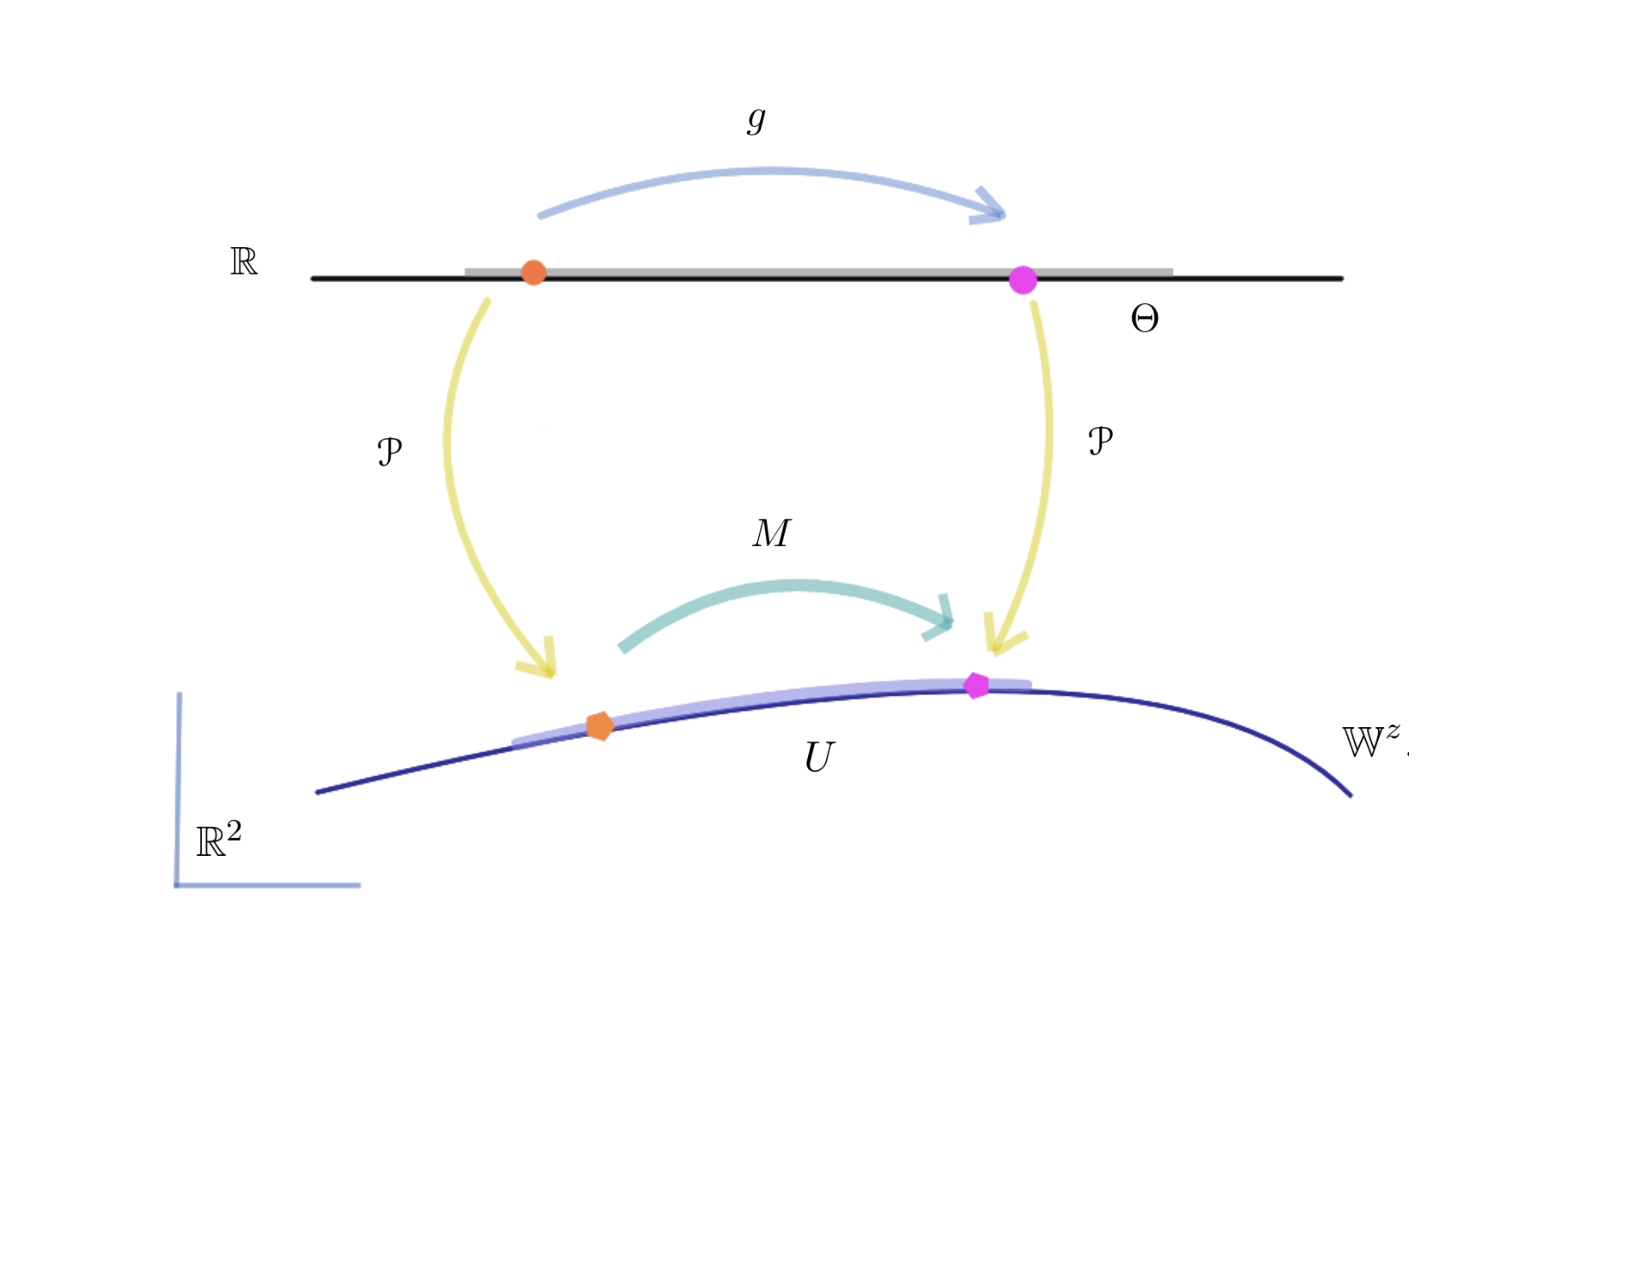
\includegraphics[scale=0.4]{diagrama2}
	\caption{Representación gr\'afica del diagrama \eqref{conmutativo}.}
	\label{diagrama-conmutativo}
\end{figure}

Las variables a encontrar en la ecuaci\'on \ref{Ecua de invariancia} son $\mathcal{P}$ y $g$, por lo que se necesita fijar o encontrar una de ellas para poder resolver la ecuaci\'on. Para hacer esto se suelen tomar en cuenta dos formas de parametrizaci\'on definidas como \textit{la forma gr\'afica} y \textit{la forma normal} \cite{Haro}. En este caso se usa la forma gr\'afica que consiste en usar la forma local de las variedades alrededor del punto $v_{*}$. Es decir se usa que localmente la dependencia es lineal, por lo que 
\begin{equation}
g(t) = \lambda t,
\label{funciong1}
\end{equation}
con $t\in \mathbb{R}$ el par\'ametro, $\lambda\in \mathbb{R}$ el valor propio asociado a la linearizaci\'on del mapeo. Esta desici\'on esta apoyada en el teorema de Hartman-Grobman \cite{devaney}\cite{Juergen}  que declara que en una vecindad del punto fijo hiperb\'olico se puede aproximar el comportamiento del sistema mediante su linearizaci\'on. \\

Entonces usando la linearizaci\'on del mapeo y la ecuaci\'on \eqref{funciong1} se puede resolver la ecuaci\'on \eqref{Ecua de invariancia} para $\mathcal{P}$. Para ello se propone que 
\begin{equation}
\mathcal{P} := (p_{1}(t), p_{2}(t)) =( \sum_{n=0}^{\infty}a_{n}t^{n}, \sum_{n=0}^{\infty}b_{n}t^{n}).
\label{polinomioecuacion}
\end{equation}
Sustituyendo la ecuaci\'on \eqref{polinomioecuacion} en la ecuaci\'on \eqref{Ecua de invariancia} se puede separar por grado de cada lado de la ecuaci\'on y comparar t\'erminos.  Las ecuaciones resultantes son recursivas , es decir que proponiendo los coeficientes de orden cero del polinomio $\mathcal{P}$ se puede obtener todos los consecutivos. 


  % ~15 pag.

%%%%%%%%%%%%%%%%%%%%%%%%%%%%%%%%%%%%%%%%%%%%%%%%%%%%%%%%%%%%%%%%%%%%%%%%%
%           Capítulo 2: MARCO TEÓRICO - REVISIÓN DE LITERATURA
%%%%%%%%%%%%%%%%%%%%%%%%%%%%%%%%%%%%%%%%%%%%%%%%%%%%%%%%%%%%%%%%%%%%%%%%%
\chapter{Implementaci\'on del m\'etodo}
En este cap\'itulo se describe brevemente c\'omo se implement\'o el m\'etodo para encontrar puntos fijos. Sobre el m\'etodo de la parametrizaci\'on implementado se puede revisar la referencia \cite{eve} en donde se describe tambi\'en c\'omo se aplic\'o al mapeo est\'andar. 

\section{Desarrollo explícito para el mapeo estándar}

El mapeo et\'andar es uno de los mapeos m\'as estudiados, esta dado por 

\begin{equation}
M_{\kappa}(x_{n},y_{n}) = 
\left(\begin{array}{c}
x_{n} +y_{n+1} \\
y_{n}-\kappa\sin(2\pi x_{n})/2\pi
\end{array}\right),
\label{mapeo estandar}
\end{equation}
con $\kappa$ un par\'ametro y $x\in [0,1]$. Escrito de esta forma el mapeo se descompone en el producto de dos involuciones dadas por
\begin{equation}
I_{0}\left( \begin{array}{c}
x_{n}\\
y_{n}
\end{array}\right) = 
\left(\begin{array}{c}
-x_{n}\\
y_{n}-\frac{\kappa}{2\pi}\sin(2\pi x_{n})
\end{array}
\right),
\label{involucionA}
\end{equation}
\begin{equation}
I_{1}\left( \begin{array}{c}
x_{n}\\
y_{n}
\end{array}\right) = 
\left(\begin{array}{c}
y_{n}-x_{n}\\
y_{n}
\end{array}
\right).
\label{involucionB}
\end{equation}

Los conjuntos invariantes asociados a las involuciones \eqref{involucionA}, \eqref{involucionB} son los siguientes
\begin{equation}
\mathbb{J}_{0} = \{ x \in [0,1] |x=0, x=1/2\},
\label{invariantejA}
\end{equation}

\begin{equation}
\mathbb{J}_{1} = \{ x \in [0,1] |x=\frac{y}{2}, x=\frac{y+1}{2}\}.
\label{invariantejB}
\end{equation}

Siguiendo el resultado del Corolario 1, sea $(x_{0},y_{0})\in \mathbb{J}_{0}$ si buscamos una \'orbita de periodo dos tendremos que resolver 
\begin{equation*}
M_{\kappa}(x,y) = M_{\kappa}(0,y)=(1/2,y),
\end{equation*}
lo cual se reduce a que
\begin{equation*}
y=1/2.
\end{equation*}
Entonces afirmamos que el punto $(0,1/2)$ es un punto de periodo dos, cuya \'orbita encontrada es $\{(0,1/2), (1/2,1/2)\}$. Es importante recordar que la variable $x$ est\'a definida en el intervalo $[0,1]$ por lo que se debe tomar m\'odulo 1 en esa componente. \\

Una vez encontrada un \'orbita peri\'odica es necesario determinar la estabilidad de la misma. Usando la linearizaci\'on alrededor del punto fijo, en este caso un punto en la \'orbita se toma como punto fijo  del mapeo  $M^{n}_{k}(x_{0},y_{0})=(x_{0},y_{0})$. La estabilidad est\'a dada por los valores propios del jacobiano $DM^{n}_{\kappa}(x_{0},y_{0})$. Para calcular este jacobiano no hace falta hacer la composici\'on, solo hace falta usar la regla de la cadena y la \'orbita peri\'odica.
\begin{align*}
DM^{n}_{\kappa}(x_{0},y_{0}) &= D(M_{\kappa}(M_{\kappa}(\cdots M_{\kappa}(x_{0},y_{0}))))\\
& = DM_{\kappa}(M^{n-1}(x_{0},y_{0}))DM_{\kappa}(M^{n-2}_{\kappa}(x_{n-2},y_{n-1}))\cdots DM_{\kappa}(x_{0},y_{0})\\
& = DM_{\kappa}(x_{n-1},y_{n-1})DM_{\kappa}(x_{n-2},y_{n-2})\cdots DM_{\kappa}(x_{0},y_{0}).
\end{align*}
Entonces el jacobiano $DM^{n}_{\kappa}(x_{0},y_{0})$ se puede calcular evaluando el jacobiano del mapeo est\'andar en los puntos de la \'orbita y multiplicando las matrices. El jacobiano del mapeo est\'andar es
\begin{eqnarray}
M^{n}_{k}(x_{n},y_{n})=\begin{pmatrix}
1 & 1 \\
- \kappa\cos(2\pi x_{n})& 1\\ 
\end{pmatrix},
\label{jacobiano mapeo}
\end{eqnarray}
y la \'orbita se conoce si se conoce solo uno de los puntos. Usando el hecho de que el determinante del producto es el producto de los determinantes se tiene que 
\begin{equation}
\textrm{det}DM^{n}_{\kappa}(x_{0},y_{0}) = \left(\textrm{det} DM(x_{n-1},y_{n-1})\right) \cdots \left(\textrm{det} DM(x_{0},y_{0})\right).
\label{determinante jacobiano m}
\end{equation} 
Si los valores propios asociados al polinomio caracter\'istico de la ecuaci\'on \eqref{determinante jacobiano m} tienen m\'odulo mayor que uno y menor que uno entonces tenemos que $(x_{0},y_{0})$ es un punto hiperb\'olico lo que indica que la \'orbita encontrada es hiperb\'olica. \\

Una vez que se tiene calculada una \'orbita peri\'odica hiperb\'olica del mapeo se aplica el m\'etodo de la parametrizaci\'on para describir las variedades invariantes asociadas a tal \'orbita. \\



Para el m\'etodo de parametrizaci\'on escribimos las variables ($x,y$) como dos polinomios de variable real $t$
\begin{eqnarray}
x(t)=\sum_{n=0}^{\infty}a_{n}t^{n}  ,
\label{x}
\end{eqnarray}
\begin{eqnarray}
y(t)=\sum_{n=0}^{\infty}b_{n}t^{n},
\label{y}
\end{eqnarray}
d\'onde $a_{0},b_{0}$ representan los coeficientes n-\'esimos del polinomio y tal que $\mathcal{P}(t):=(x(t),y(t))$. En cuanto a la dinámica interna $g$, se usa la ecuación $g(t)=\lambda t$ \eqref{funciong1}. Sustituyendo las variables en su expansi\'on de Taylor en $M\circ\mathcal{P}=\mathcal{P}\circ g$ \eqref{Ecua de invariancia}  y usando que $M$ es el mapeo est\'andar \eqref{mapeo estandar} obtenemos
\begin{eqnarray}
M_{\kappa}(x,y) = \left[\begin{array}{c}
x(t) + y(t) -\frac{\kappa}{2\pi}\sin(2\pi x(t)) \\
y(t) - \frac{\kappa}{2\pi}\sin[2\pi x(t)]
\end{array}\right] =\left[ \begin{array}{c}
x(\lambda t) \\
y(\lambda t)
\end{array}\right], 
\label{sumas en mapeo}
\end{eqnarray}
que en forma explícita es
\begin{eqnarray}
\left[\begin{array}{c}
\sum_{n=0}^{\infty}a_{n}t^{n} + \sum_{n=0}^{\infty}b_{n}t^{n} -\frac{\kappa}{2\pi}\sin\left(2\pi \sum_{n=0}^{\infty}a_{n}t^{n}\right)\\
\sum_{n=0}^{\infty}b_{n}t^{n} - \frac{\kappa}{2\pi}\sin(\sum_{n=0}^{\infty}b_{n}t^{n})
\end{array}\right] =\left[ \begin{array}{c}
\sum_{n=0}^{\infty}a_{n}\lambda^{n}t^{n} \\
\sum_{n=0}^{\infty}b_{n}\lambda^{n}t^{n}
\end{array}\right].
\label{expandida}
\end{eqnarray}
al desarrollar las sumas y usar la serie de Taylor del seno se puede obtener una ecuaci\'on para comparar los t\'erminos de \'orden 0. 

\begin{align*}
	\left[
	\begin{array}{c}
		\sum_{n=0}^{\infty}a_{n}t^{n} + \sum_{n=0}^{\infty}b_{n}t^{n}-\frac{\kappa}{2\pi}\sum_{n=0}^{\infty}\frac{(-1)^{n}}{(2n+1)!}\left(2\pi \sum_{n=0}^{\infty}a_{n}t^{n}\right)^{2n+1}\\
		\sum_{n=0}^{\infty}b_{n}t^{n}-\frac{\kappa}{2\pi}\sum_{n=0}^{\infty}\frac{(-1)^{n}}{(2n+1)!}\left(2\pi\sum_{n=0}^{\infty}a_{n}t^{n}\right)^{2n+1}
	\end{array}	\right]
	&=\\
	\left[
	\begin{array}{c}
		\sum_{n=0}^{\infty}a_{n}\lambda^{n}t^{n} \\
		\sum_{n=0}^{\infty}b_{n}\lambda^{n}t^{n}
	\end{array}
	\right]
\end{align*}
Desarrollando las sumas y agrupando los t\'erminos de \'orden cero.
\begin{equation}
	\left[
	\begin{array}{c}
	
			a_{0}+b_{0}-\frac{\kappa}{2\pi}\left(2\pi a_{0}-\frac{2\pi}{3!} 	a_{0}^{3}+\frac{2\pi}{5!} a_{0}^{5}-\cdots
			\right)\\
			b_{0}-\frac{\kappa}{2\pi}\left(2\pi a_{0}-\frac{2\pi}{3!}a_{0}^{3}+\frac{2\pi}{5!}a_{0}^{5}-\cdots\right)
	\end{array}
	\right]=
	\left[
	\begin{array}{c}
		a_{0}\\
		b_{0}
	\end{array}
	\right]
\end{equation}
De donde se obtiene que $a_{0},b_{0}$ son cero. An\'alogamente se pueden agrupar los de primer orden y obtener un sistema que se resuelve a partir de los coeficientes $a_{0}$ y $b_{0}$. De manera sucesiva se pueden obtener ecuaciones de recurrencia para encontrar los coeficientes de orden $j$, los detalles de c\'omo son estos c\'alculos se pueden consultar en \cite{eve}.


\section{Implementación del método}
La implementaci\'on del m\'etodo consiste principalmente en aplicar un m\'etodo de Newton para encontrar ra\'ices. Para encontrar las \'orbitas peri\'odicas, dado el mapeo y los conjuntos invariantes de las simetr\'ias se puede buscar una \'orbita peri\'odica de periodo $n$ usando una semilla. En la siguiente tabla se ezquematiza c\'omo se calcula, sin embargo se recomienda que para mayor detalle viste \url{https://github.com/alvarezeve/Tesis-Variedades-Estables-e-inestables/}.
En la liga se encuentra la documentaci\'on necesaria para poder usar el m\'etodo as\'i como algunos ejemplos. \\
\linebreak
\linebreak
\linebreak
\begin{center}
	\textcolor{blue}{\textbf{Pasos}}
	\begin{tabbing}
	12\=1234567890123456789012345678901234567890123456\=12345678901234567890123456\kill%
	\>............................................................  \>..................................................\\
	\>\textbf{1.}  Se reciben el mapeo, las involuciones,  \> \\
	\>el periodo y una semilla. \>$M, I_{A}, I_{B},n,v_{0}$ \\
	\>............................................................  \>..................................................\\
	\>\textbf{2.} Se crea un nuevo mapeo que es \> \\
	\> la composición del mapeo $M$, $k$ veces.\>  $f(v)=M^{k}(v)$ \\
	\>............................................................  \>..................................................\\
	\>\textbf{3.} Se toma un punto en el conjunto  \> $J_{A}$\\
	\> invariante. \> \\
	\>............................................................  \>..................................................\\
	\>\textbf{4.} Se usa la función creada en el paso 2. \> \\
	\> y se aplica al punto elegido en el paso \> $f(p)$\\
	\> anterior.\> \\
	\>............................................................  \>..................................................\\
	\>\textbf{5.} Se usa la ecuación que describe \> \\
	\> el conjunto $J_{B}$ y el hecho de que es  \> $g(f(p))=0$\\
	\>invariante para construir una nueva  \> \\
	\> ecuación.\\
	\>............................................................  \>..................................................\\
	\>\textbf{6.}  Se usa un método de Newton para \> \\
	\> encontrar la raíz de la ecuación del \> \\
	\> paso 5.\\
	\>............................................................  \>..................................................\\
	\end{tabbing} 
\end{center}

La implementaci\'on del m\'etodo de parametrizaci\'on fue resultado de un trabajo anterior \cite{eve}, por lo que solo se decribir\'a de manera muy superficial lo programado. Al igual que en el caso del m\'etodo para las \'orbitas peri\'odicas se puede encontrar la documentaci\'on en  \url{https://github.com/alvarezeve/PeriodicOrbits2DMaps}. 

\begin{center}
	\textcolor{blue}{\textbf{Pasos}}
	\begin{tabbing}
		12\=1234567890123456789012345678901234567890123456\=12345678901234567890123456\kill%
		\>............................................................  \>..................................................\\
		\>\textbf{1.} Se reciben el mapeo, el punto fijo  \> \\
		\> el orden del polinomio, el intervalo en  \> $M, O, v, t, \Delta t$\\
		\> el que se va a evaluar y el paso.\> \\
		\>............................................................  \>..................................................\\
		\>\textbf{2.} Se crean dos polinomios de grado 1  \> $P_{x} = a_{0}+a_{1}t+O(t^{2})$\\
		\> asociados a las variables del mapeo. \>  $P_{y} = b_{0} +b_{1}t+O(t^{2})$ \\
		\>............................................................  \>..................................................\\
		\>\textbf{3.} Se aplica el mapeo a los polinomios.  \> $M(P_{x}+P_{y})$\\
		\>............................................................  \>..................................................\\
		\>\textbf{4.} Se calcula la matriz jacobiana del  \> \\
		\>sistema anterior y se calculan los valores \> $JM(P_{x},P_{y})$\\
		\> y vectores propios.\\
		\>............................................................  \>..................................................\\
		\>\textbf{5.} Se elige el valor propio asociado a la  \> \\
		\>variedad que se está calculando \> $\lambda$\\
		\>............................................................  \>..................................................\\
		\>\textbf{6.}Se resuelve para $a_{1},b_{1}$.\> $a_{1}(a_{0}, \lambda), b_{1}(b_{0},\lambda)$\\
		\> \> \\
		\>............................................................  \>..................................................\\
		\> \textbf{7. }Se sustituyen los valores de $a_{1},b_{1}$ \> $P_{x} = a_{0}+a_{1}t+a_{2}t^{2}+O(t^{3})$\\
		\> en los polinomios $P_{x},P_{y}$ y se aumenta\>  $P_{y} = b_{0} +b_{1}t +b_{2}t^{2}+O(t^{3})$\\
		\>  el orden.\> \\
		\>............................................................  \>..................................................\\
		\>\textbf{8.} Se aplica el mapeo a los nuevos\>$M(P_{x}+P_{y})$ \\
		\> polinomios.\>\\
		\>............................................................  \>..................................................\\
		\>\textbf{9.} Se crea el polinomio. \> $P_{\lambda x} = a_{0}+a_{1}\lambda t+a_{2}\lambda t^{2}+O(t^{3})$\\
		\> \>$P_{\lambda y} = b_{0}+b_{1}\lambda t+b_{2}\lambda t^{2}+O(t^{3})$\\
		\>............................................................  \>..................................................\\
		\>\textbf{10.} Se crea una ecuación con la resta \> $M(P_{x}+P_{y}) -(P_{\lambda x},P_{\lambda y})$=0 \\
		\> de las ecuaciones del paso 8 y 9.\> \\
		\>............................................................  \>..................................................\\
		\> \textbf{11.} Se resuelve la ecuación del paso 10 \>  \\
		\> para las variables $a_{2},b_{2}$. \>\\
		\>............................................................  \>..................................................\\
		\> \textbf{12.} Se regresa al paso 7 y se itera\> \\
		\> hasta que se llegue al orden deseado. \> \\
		\>............................................................  \>..................................................\\
		
		
		
		
	\end{tabbing} 
\end{center}


En ambas implementaciones se añadi\'o una forma de evaluar el error num\'erico. Para las \'orbitas peri\'odicas se tom\'o la diferencia entre el punto de la \'orbita de periodo $n$ encontrado y su n-\'esima iteraci\'on.
\begin{equation}
	\mathbb{E} = ||(x_{0},y_{0})-M^{n}(x_{0},y_{0})||
	\label{errororbitasperiodicas}
\end{equation}
Mientras que en el caso de las parametrizaciones el error se toma de la diferencia entre composiciones evaluada en el intervalo en el que se tom\'o la parametrizaci\'on  \cite{Mireles}. 
\begin{equation}
	\mathbf{E} = || M\circ \mathcal{P}- \mathcal{P}\circ g||
\end{equation}
Los errores se analizan por separado ya que cada m\'etodo puede considerarse ajeno. 






   

%%%%%%%%%%%%%%%%%%%%%%%%%%%%%%%%%%%%%%%%%%%%%%%%%%%%%%%%%%%%%%%%%%%%%%%%%
%           Capítulo 3: Mapeo de Hénon
%%%%%%%%%%%%%%%%%%%%%%%%%%%%%%%%%%%%%%%%%%%%%%%%%%%%%%%%%%%%%%%%%%%%%%%%%
\chapter{Resultados}
%\label{SeccionEstandar}\section{Mapeo estándar}

Utilizando el método ya programado se hicieron diferentes cálculos para encontrar algunas \'orbitas peri\'odicas en el mapeo est\'andar, que se muestran en la figura \ref{orbitasperiodicasestandarv}. Todas las \'orbitas que aparecen fueron calculadas n\'umeros de tipo \textrm{Float64} y presentan un error menor al $1\times10^{-15}$.
\begin{figure}[H]
	\centering
	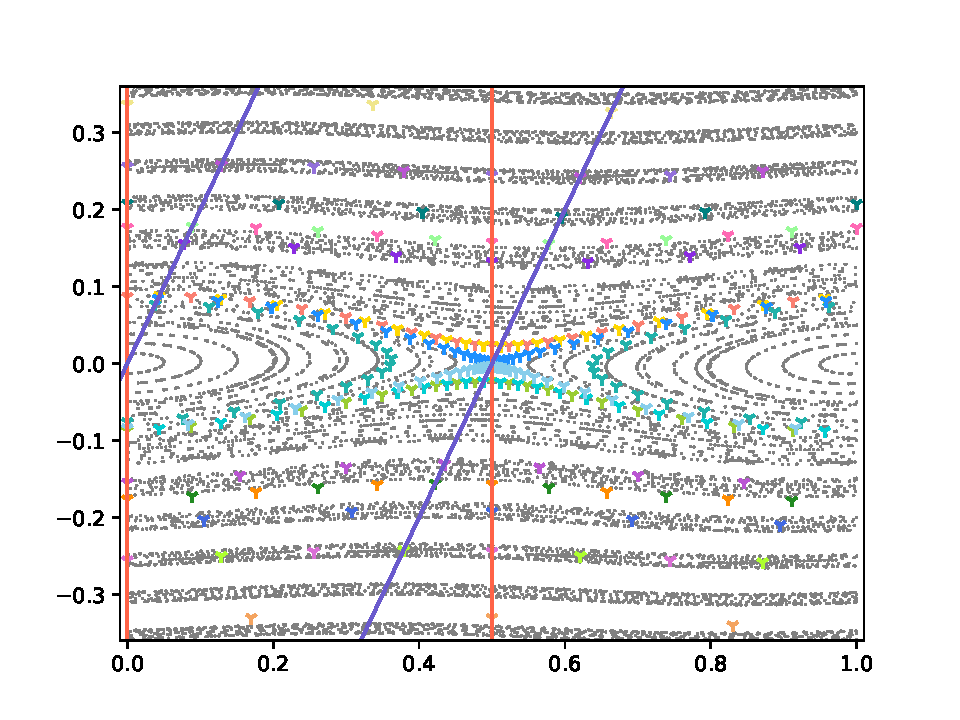
\includegraphics[scale= 0.7]{EstandarOP07}
	\label{orbitasperiodicasestandarv}
	\caption{Espacio fase del mapeo est\'andar, con $\kappa = 0.07$, junto con varias \'orbitas peri\'odicas. Las lineas rojas y azul representan los conjuntos invariantes $\mathbb{J}_{0},\mathbb{J}_{1}$}.
\end{figure}
\begin{figure}[H]
	\centering
	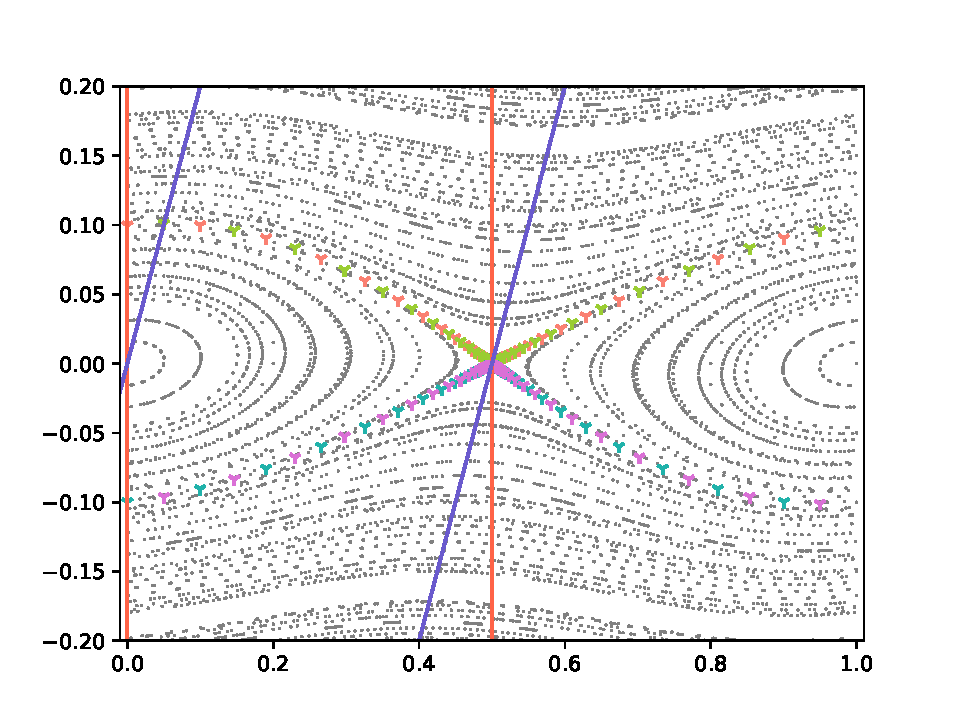
\includegraphics[scale= 0.7]{EstandarOP1-40.pdf}
	\label{orbitasp40estandar}
	\caption{Espacio fase del mapeo est\'andar, con $\kappa = 0.07$, con 4  \'orbitas de periodo 40. Las lineas rojas y azul representan los conjuntos invariantes $\mathbb{J}_{0},\mathbb{J}_{1}$}. 
\end{figure}

Para caclular las \'orbitas se requiere una semilla para iniciar el m\'etodo de Newton, esta semilla se calcul\'o primero calculando las \'orbitas peri\'odicas del mapeo cuando el valor del par\'ametro es $\kappa=0.0$ y el sistema es completamente integrable. \\ 

Otro mapeo con el que se trabaj\'o fue el mapeo cuadr\'atico que es una mapeo que preserva \'area y donde $a,b$ son n\'umeros reales. El mapeo es integrable cuando $b=0$.
\begin{equation}
	M_{a,b}(x_{n},y_{n}) = \left(
	\begin{array}{c}
	x_{n}+a(1-y_{n+1}^{2})\\
	y_{n}-b\sin(2\pi x_{n})
	\end{array}
	\right)
	\label{mapeocuadratico}
\end{equation}
Sus correspondientes involuciones son.
\begin{equation}
	\mathbf{I}_{0}
	\left(\begin{array}{c}
		x\\
		y
	\end{array}
	\right) = 
	\left(-x\\
	y-b\sin(2\pi x)
	\right)
	\label{involucioncuadratico0}
\end{equation}
\begin{equation}
	\mathbf{I}_{1}
	\left(\begin{array}{c}
		x\\
		y
	\end{array}
	\right) = 
	\left(-x+ a(1-y^{2})\\
	y
	\right)
	\label{involucioncuadratico1}
\end{equation}

Mientras que sus conjuntos invariantes asociados son
\begin{equation}
	\mathbb{J}_{0} = \{ (x,y) | x=0 ,x=1/2\}
	\label{conjunto invariante cuadratico 0}
\end{equation}
\begin{equation}	
	\mathbb{J}_{1} = \{ (x,y)| x= a(1-y^{2})/2, x = a(1-y^{2})/2+1/2
		\}
	\label{conjunto invariante cuadratico 1}
\end{equation}
Utilizando el m\'etodo implementado de la misma manera que se utiliz\'o para el mapeo est\'andar es posible obtener \'orbitas peri\'odicas de diferentes periodos usando semillas adecuadas. Un ejemplo de algunas \'orbitas se muestra en la figura \ref{grafmapeocuadratico1}. \\

\begin{figure}[H]
	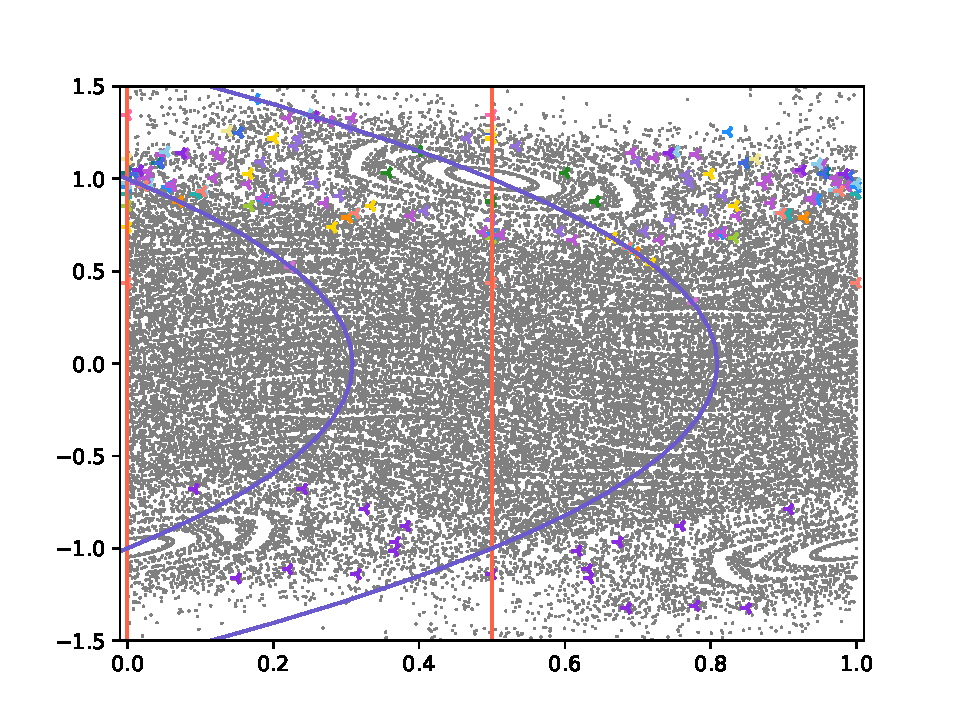
\includegraphics[scale=0.7]{MapeoCuadraDifP}
	\label{grafmapeocuadratico1}
	\caption{Espacio fase y algunas \'orbitas peri\'odicas del mapeo \eqref{mapeocuadratico} con $ a = 0.618, b=0.2$. Las curvas de color rojo y azul corresponden a los conjuntos $\mathbb{J}_{0}, \mathbb{J}_{1}$.} 
\end{figure}
\begin{figure}
	\centering
	\includegraphics[scale=0.6]{MApeoCP4A}
	\caption{\'Orbita de periodo 4 en el mapeo \eqref{mapeocuadratico} con $a = 0.2625, b = 0.44$.}
	\label{grafmapeocuadraper4}
\end{figure}
Es posible dentro del programa implementado cambiar el m\'etodo para encontrar las ra\'ices dentro del m\'etodo. Sin embargo es mejor encontrar la forma de obetener ra\'ices que se aproximen a un punto de la \'orbita  ya que eso garantiza la convergencia del m\'etodo usando los m\'etodos de soluci\'on de ra\'ices m\'as simples. Tambi\'en se implement\'o una extensi\'on del m\'etodo para aritm\'etica de presici\'on extendida. En presici\'on extendida se utilizan n\'umeros de presici\'on arbitraria la cual trabaja con 256 bits predefinida. \\

Algo interesante de analizar con est\'a herramienta es la din\'amica de las \'orbitas peri\'odicas con forme se mueven los par\'ametros. En el caso del mapeo \eqref{mapeocuadratico} se muestra en la figura  \ref{grafmapeocuadraper4variable} c\'omo la \'orbita de periodo 4 se va modificando al variar el par\'ametro $b$ y dejando fijo $a=0.618$.

\begin{figure}[H]
	\centering
	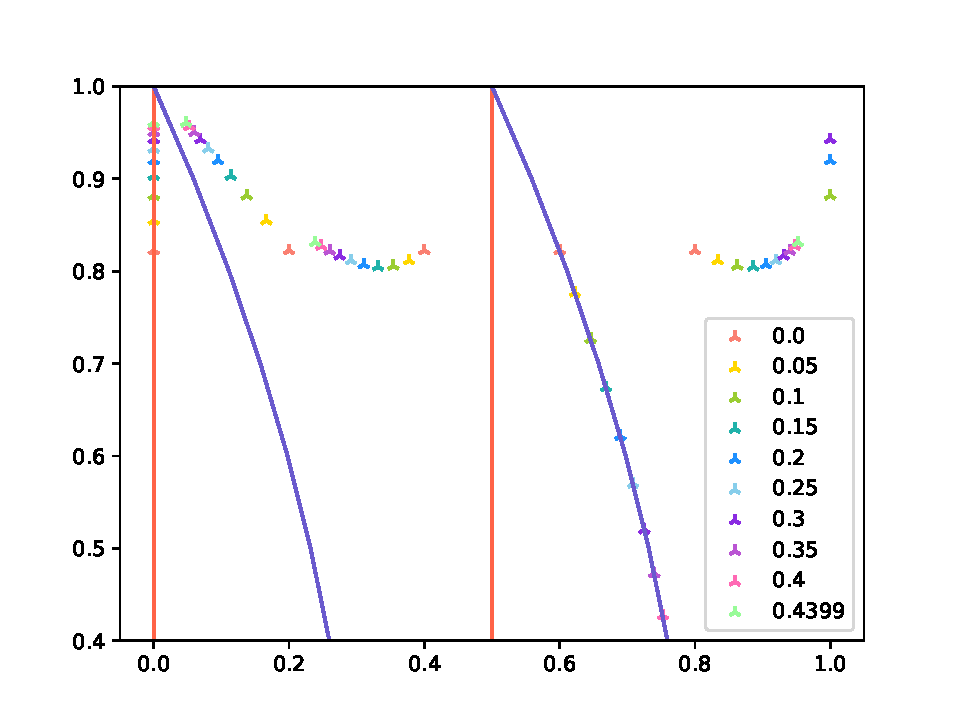
\includegraphics[scale=0.7]{MapeoCuadraP5b}
	\caption{Din\'amica de una \'orbita de periodo 4 del mapeo \eqref{mapeocuadratico} con valores $a=0.618$ fija y $b$ variable. Las curvas rojas y azules corresponden a los conjuntos invariantes $\mathbb{J}_{0}, \mathbb{J}_{1}$. }
	\label{grafmapeocuadraper4variable}
\end{figure}

\section{\'Orbitas peri\'odicas hiperb\'olicas y sus variedades.}
Una vez que se tienen algunas \'orbitas peri\'odicas es posible determinar cu\'ales de ellas son hiperb\'olicas. Seleccionando las que cumplan ser hiprb\'olicas es posible ahora aplicar el m\'etodo de parametrizaci\'on para las variedades asociadas a la \'orbita. \\

En el caso del mapeo est\'andar es bien conocido que existe una \'orbita hiperb\'olica de periodo 2 que persiste para ciertos valores del par\'ametro $\kappa$. Usando diferentes valores del par\'ametro se calcularon las parametrizaciones de las variedades asociadas usando polinomios de orden $70$ evaluados en el intervalo $t=[-0.2,0.2]$. La figura \ref{estandarvariedadesperiodo2} muestra las variedades en el espacio fase asociadas a la \'rbita hiperb\'olica de periodo dos para diferentes valores de $\kappa$. Como s epuede observar mientras el valor de $\kappa$ aumenta las variedades se van abriendo dejando mayor espacio a la din\'amica de la \'orbita el\'iptica de periodo dos. \\



\begin{figure}
	\centering
	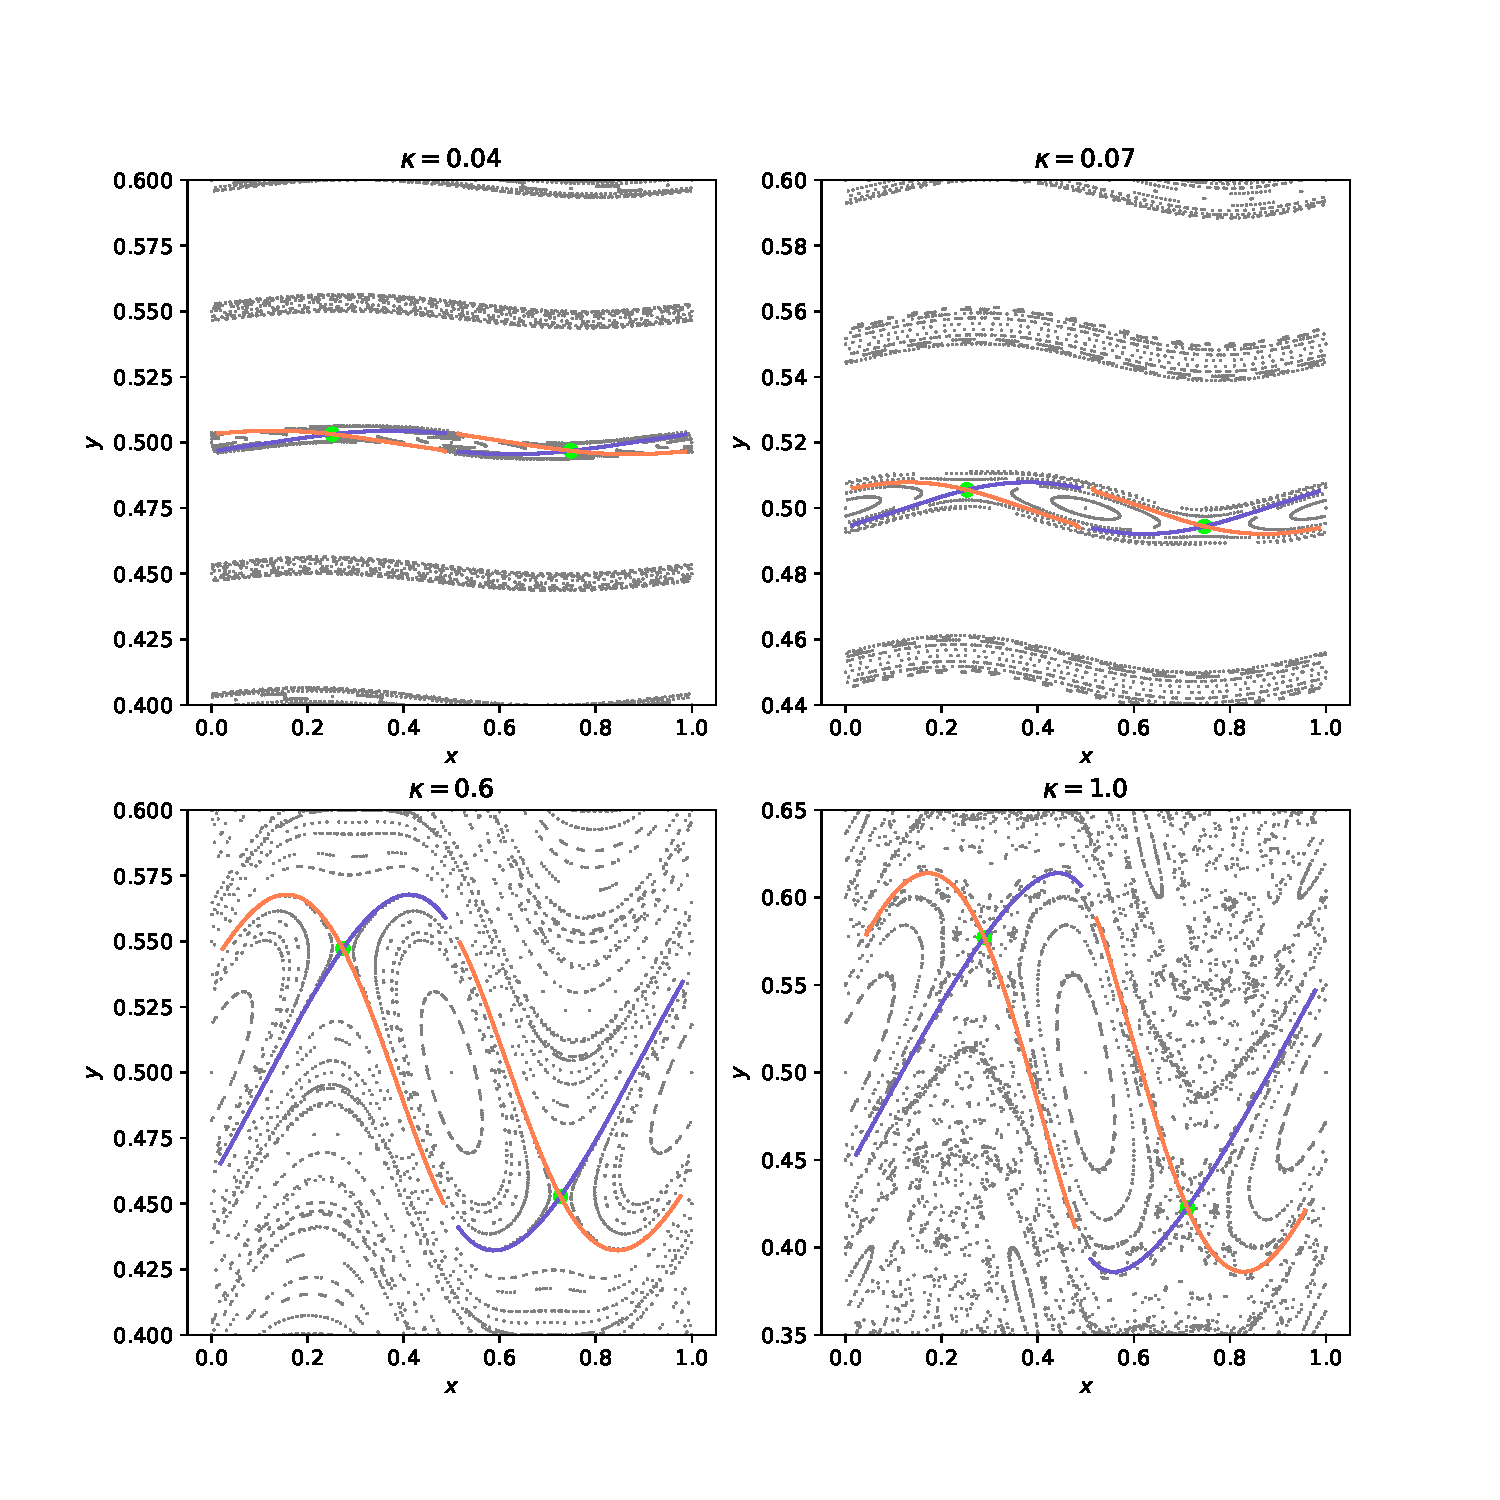
\includegraphics[scale=0.6]{variedadesestandarperiodo2}
	\caption{Variedades invariantes asociadas a la \'orbita de periodo dos en el mapeo est\'andar con diferentes valores de $\kappa$.}
	\label{estandarvariedadesperiodo2}
\end{figure}
\begin{figure}
	\centering
	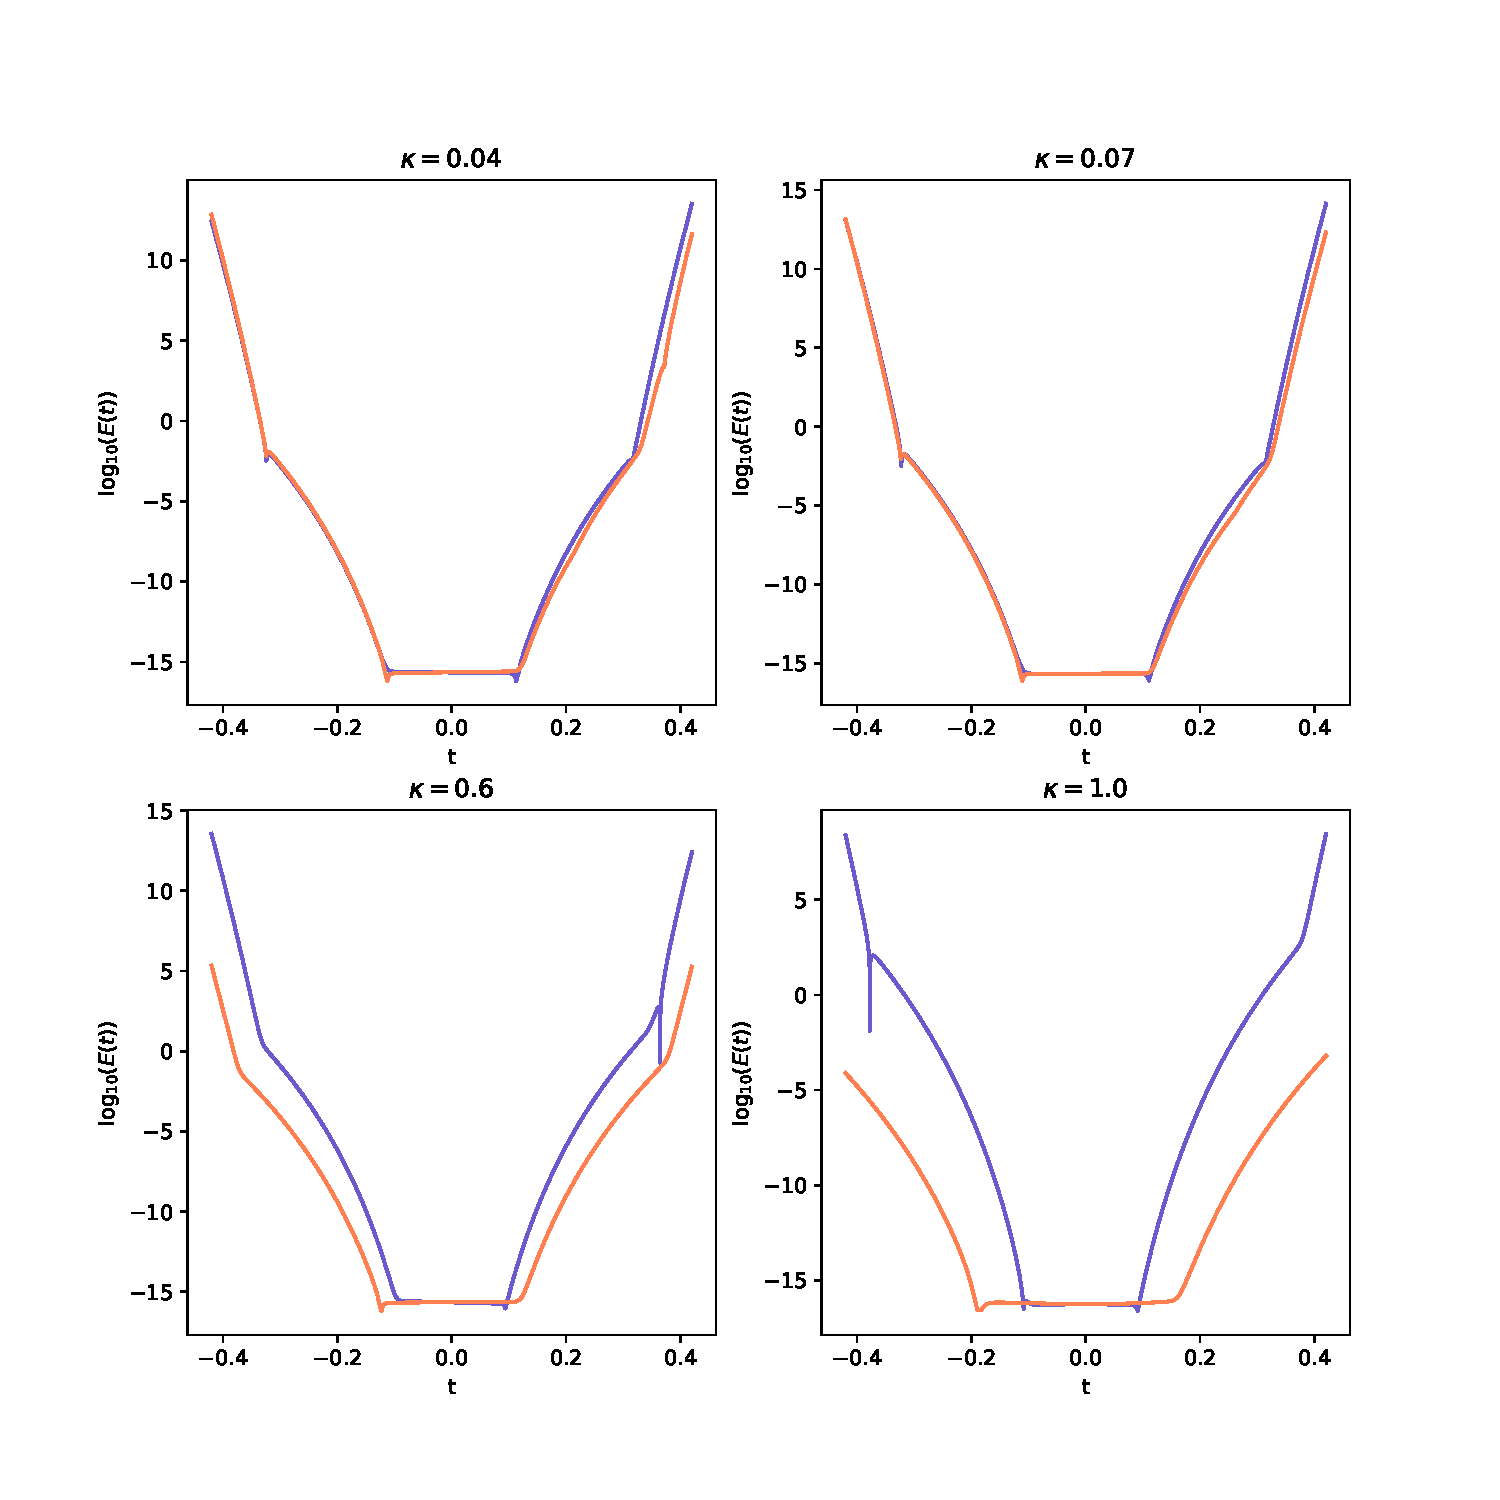
\includegraphics[scale=0.7]{erroresvariedadesestandarperiodo2}
	\caption{Errores asociados al c\'alculo de las variedades invariantes que aparecen en la figura \ref{estandarvariedadesperiodo2}.}
	\label{erroresvariedadesestandarperiodo2}
\end{figure}
Variando el valor de $\kappa$ entre $0.1$ y $1.1$ y calculando las \'orbitas hiperb\'olicas de periodo dos y sus respectivas variedades se obtuvo la figura  \ref{variedadesestandarkappasv} donde se muestra como la \'orbita de periodo dos se va deformando as\'i como las variedades. De cada punto marcado en color verde surge una variedad estable (verde) y una variedad inestable (naranja), se puede notar como la variedad estable se convierte en la inestable del punto siguiente en la \'orbita.\\

En la tabla 1 se muestra el error asociado al c\'alculo de la \'orbita peri]'odica que se obtuvo mediante la ecuaci\'on  \eqref{errororbitasperiodicas}, mientras que en la figura \ref{erroresvariedadesestandarperiodo2} se muestra el error asociado al c\'aclulo de las variedades invariantes. Como se puede observar despu\'es el error crece r\'apidamente despu\'es de un valor del par\'ametro que depende de cada parametrizaci\'on. Por esa raz\'on las variedades que aparecen en la figura \ref{estandarvariedadesperiodo2} fueron calculadas en los intervalos donde el error es m\'inimo, es decir menor a  un orden $10^{-10}$. 

\begin{center}
\begin{table}[H]
	\centering
	\begin{tabular}{|c|c|}
		\hline
		$\kappa$&  Error  \\
		\hline
		$0.01$ &  $2.220446049250313e-16$\\
		\hline
		$0.02$& $0.0$ \\
		\hline
		$0.03$	& $2.220446049250313e-16$  \\
		\hline
		$0.04$&  $2.220446049250313e-16$\\
		\hline
		$0.05$&  $2.220446049250313e-16$\\
		\hline
		$0.06$&  $2.220446049250313e-16$\\
		\hline
		$0.07$&  $2.220446049250313e-16$\\
		\hline
		$0.08$& $0.0$  \\
		\hline
		$0.09$& $0.0$  \\
		\hline
		$0.1$& $0.0$  \\
		\hline
		$0.2$&$3.3306690738754696e-16$  \\
		\hline
		$0.3$& $2.220446049250313e-16$ \\
		\hline
		$0.4$&$2.220446049250313e-16$  \\
		\hline
		$0.5$&$2.220446049250313e-16$  \\
		\hline
		$0.6$& $4.440892098500626e-16$ \\
		\hline
		$0.7$& $0.0$  \\
		\hline
		$0.8$& $0.0$ \\
		\hline
		$0.9$& $4.440892098500626e-16$   \\
		\hline
		$1.0$& $4.440892098500626e-16$  \\
		\hline
		$1.1$& $4.440892098500626e-16$  \\
		\hline
	\end{tabular}
\caption{Tabla con los errores asociados al c\'alculo de la \'orbita de periodo 2 en el mapeo est\'andar con diferentes valores de $\kappa$.}
\end{table}
\end{center}


En el caso del mapeo \eqref{mapeocuadratico} se aplic\'o el m\'etodo para dos \'orbitas encontradas, una de periodo 3 y una de periodo 11, tomando el valor de par\'ametro $a=0.618$  fijo y variando $b$. El error asociado a las \'robitas peri\'odicas est\'a en el mismo orden que en el caso del mapeo est\'andar, es decir menor a $10^{-10}$. Lo que podemos ver de las figuras 23423 es que cuando el par\'ametro $b$ es cercano a cero las variedades asociadas a las \'orbitas peri\'odicas resultan con menos curvaturas. Cuando el par\'ametro $b$ va aumentando las \'orbitas peri\'odicas se van acercando como se muestra en la figura 23534 en donde las \'orbitas son cercanas y sus variedades tambi\'en. Adem\'as de esto podemos obervar que las variedades se van curvando y teniendo un comportamiento m\'as complicado de describir. Cuando el valor de $b$ aumenta lo suficiente las \'orbitas est\'an lo suficientemente cerca como para que las variedades de la \'orbita de periodo tres y la de periodo once se corten en varios puntos como se puede ver en la figura 34534. \\


\begin{figure}[H]
	\centering
	\includegraphics[scale=0.5]{variedadesestandarkappas}
	\caption{Comportamiento de las variedades invariantes asociadas a la \'orbita de periodo dos en el mapeo est\'andar al variar $\kappa$ entre $[0.1,1.1]$.}
	\label{variedadesestandarkappasv}
\end{figure}

\begin{figure}[H]
	\centering
	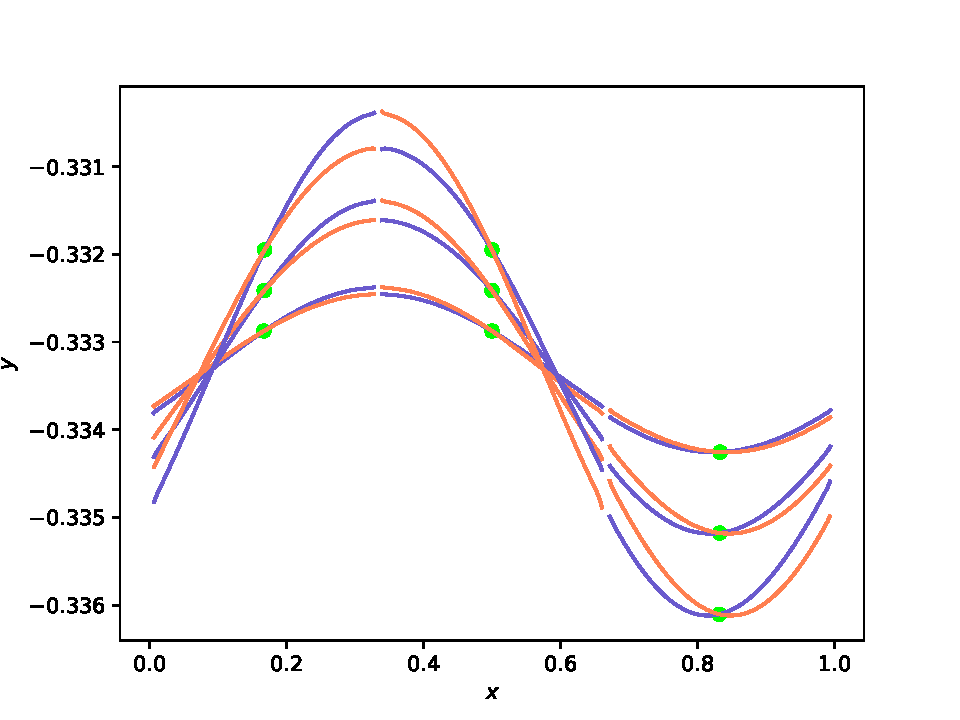
\includegraphics[scale=0.5]{variedadesestperiodo3kvar}
	\caption{Variedades asociadas a una \'orbita de periodo tres para el mapeo est\'andar con valores de $\kappa = [0.01,0.02,0.03]$. }
	\label{vairedadesperiodo3kvariable}
\end{figure}

\begin{figure}[H]
	\centering
	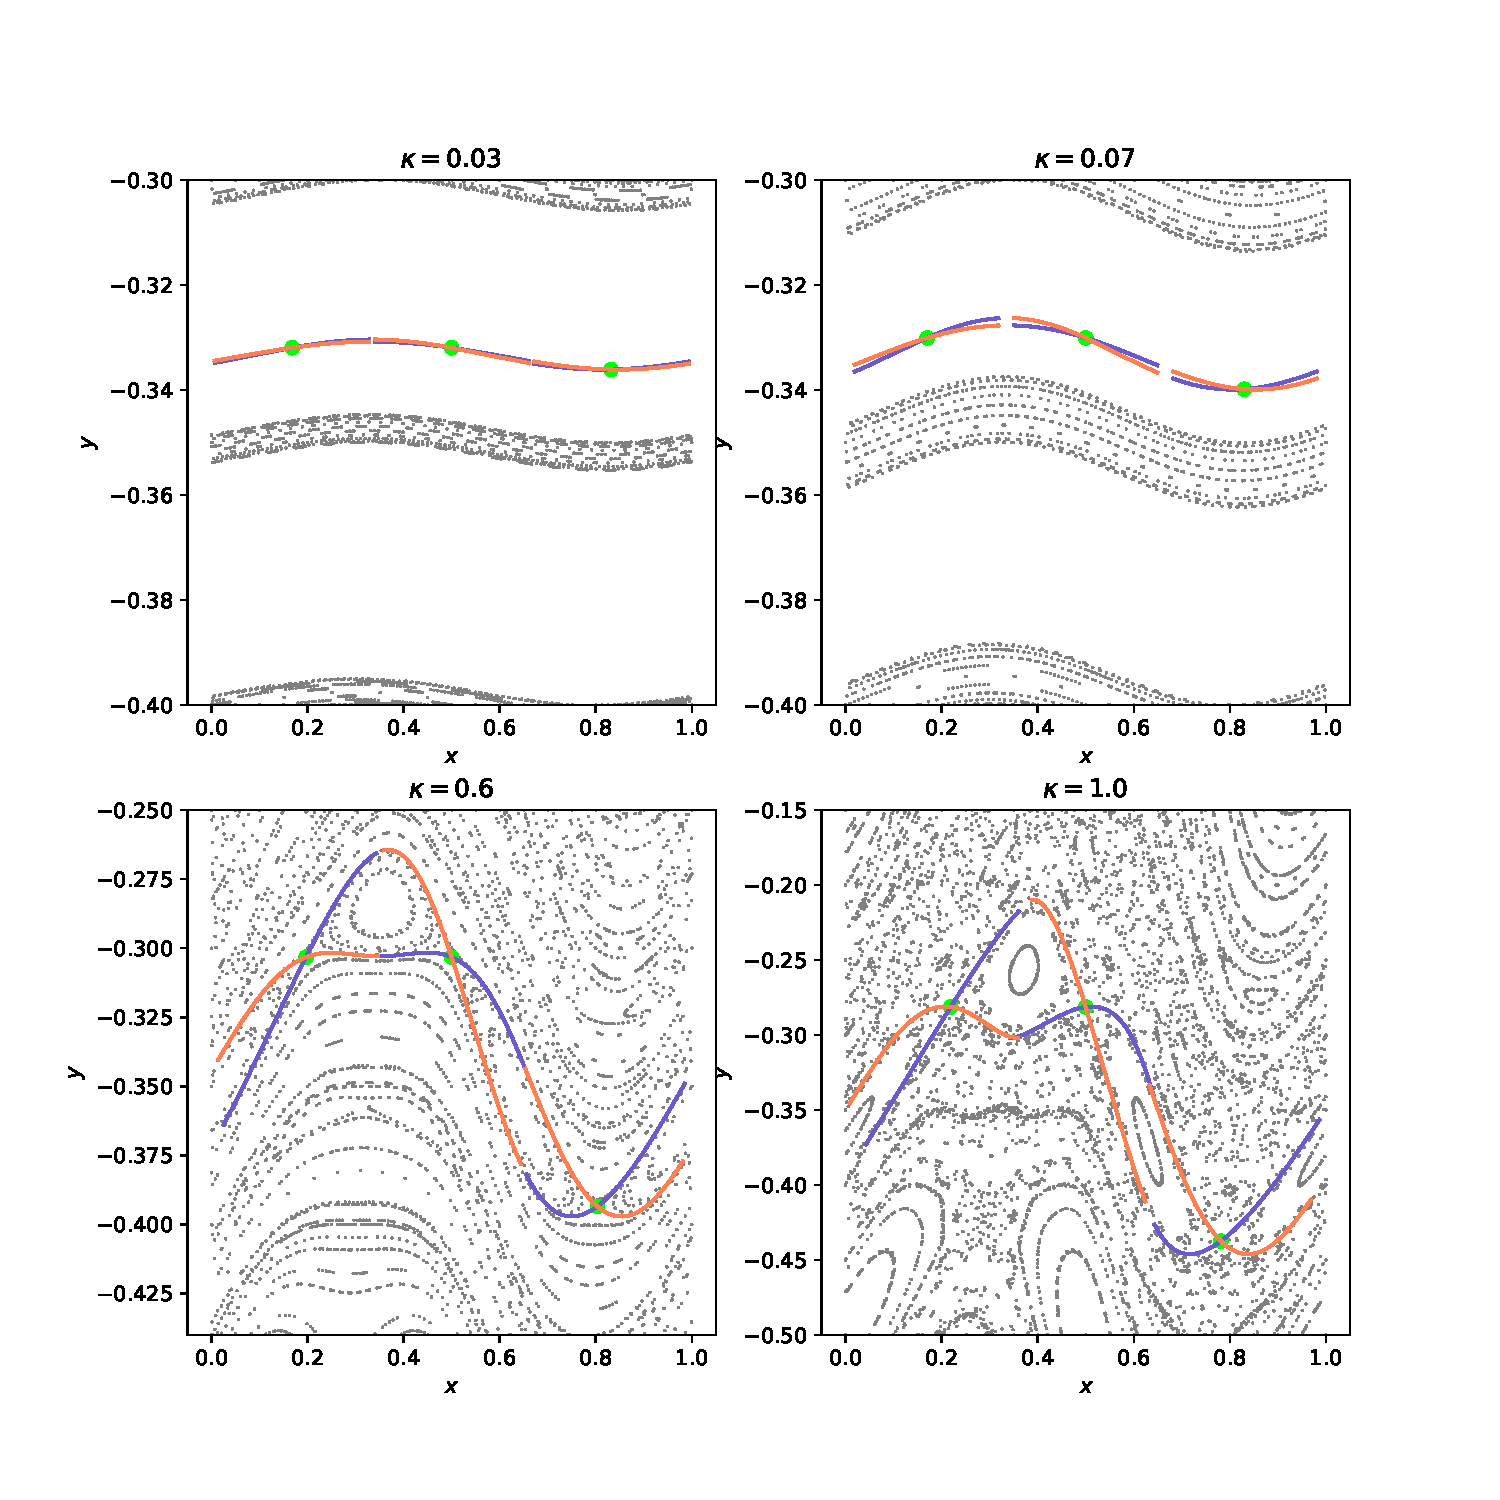
\includegraphics[scale=0.7]{variedadesestandarperiodo3}
	\caption{Variedades invariantes asociadas a una \'orbita de periodo 3 en el mapeo est\'andar con diferentes valores de $\kappa$.}
	\label{variedadesestandarperiodo3}
\end{figure}
\begin{figure}[H]
	\centering
	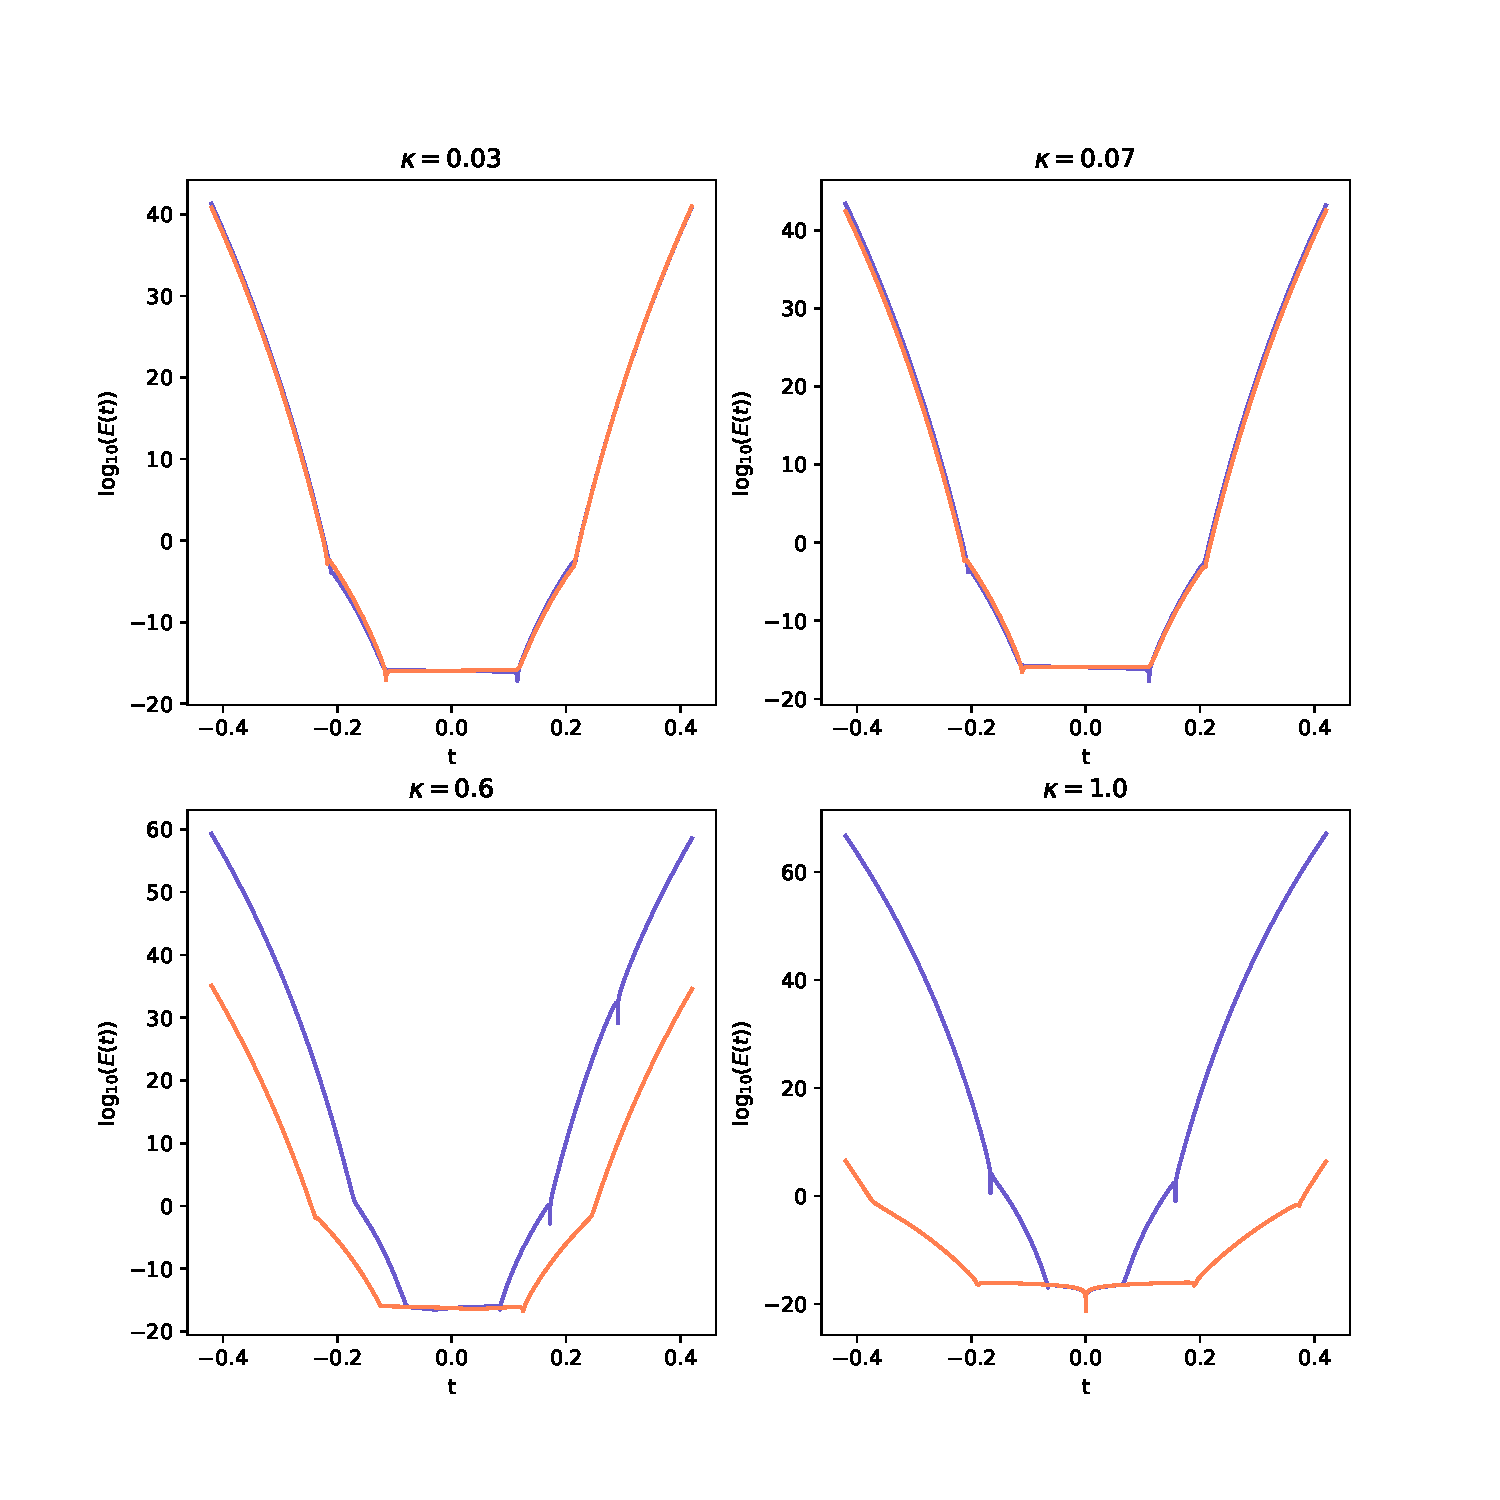
\includegraphics[scale=0.7]{erroresvariedadesestandarperiodo3}
	\caption{Errores asociados al c\'aculo de las variedades invariantes de la figura \ref{variedadesestandarperiodo3}. }
	\label{erroresvariedadesperiodo3}
\end{figure}

\begin{figure}[H]
	\includegraphics[scale=0.7]{variedadescuadraticop3p11A}
	\caption{Variedades invariantes asociadas a dos \'orbitas de periodo tres y once respectivamente, para el mapeo \eqref{mapeocuadratico}, con diferentes valores del par\'ametro $b$ y manteniendo $a$ fijo.}
	\label{variedadescuadraticoper3per11vark}
\end{figure}
\section{Conclusiones}
Mediante el m\'etodo descrito para encontrar \'orbitas peri\'odicas es posible encontrar \'orbitas de periodo $N$ en mapeos simpl\'ecticos de dos dimensiones usando una semilla adecuada. Dado que el m\'etodo usa internamente un m\'etodo para encontrar ra\'ices en una dimensi\'on es importante tener en cuenta que se cumplan los requerimentos para que el m\'etodo converga. Las instrucciones de c\'omo puede modificarse el m\'etodo o la presici\'on con la que se calculan las \'orbitas puede encontrarse en PONER URL al git. \\

Se present\'o adem\'as un m\'etodo para determinar la estabilidad de las \'orbitas encontradas. Este m\'etodo proviene de usar la regla de la cadena en la composici\'on del mapeo con el que se est\'e trabajando y del hecho de que cualqui\'er \'orbita de periodo $N$ es un punto fijo del mapeo $M^{N}$. Usando esto y la forma en la que se determina la estabilidad de un punto fijo se construy\'o el m\'etodo para determinar la estabilidad.\\

Para las \'orbitas peri\'odicas hiperb\'olicas se aplic\'o el m\'etodo de la parametrizaci\'on para describir las variedades asociadas a la \'orbita. El m\'etodo ya hab\'ia sido implementado previamente para puntos fijos hiperb\'olicos de mapeos de dos dimensiones por lo que solo fueron necesarios algunas modificaciones simples para usarlo en \'orbitas peri\'odicas. Mediante este m\'etodo fue posible describir el comportamiendo de variedades asociadas a \'orbitas per\'iodicas en cada uno de los puntos de la \'orbita.\\

El orden de la parametrizaci\'on se puede elegir y modificar para que la variedad se pueda describir con un error aceptable en alg\'un intervalo deseado. Sin embargo no es posible con solo aumentar el orden del polinomio describir una variedad en intervalos \textit{grandes} (el tamaño depende del mapeo y de la \'orbita peri\'odica), por lo que una alternativa es usar aplicar el mapeo a la parametrizaci\'on, como una especie de iteraci\'on pero no de puntos en el espacio fase, sino directamente de la expresi\'on polin\'omica de la variedad. La iteraci\'on de la variedad nos da un nuevo polinomio con diferentes coeficientes que pueden describir un intervalo mayor de la variedad. \\

Uniendo los m\'etodos fue posible observar la din\'amica de las \'orbitas peri\'odicas y de las variedades asociadas cuando el par\'ametro $\kappa$ en el mapeo est\'andar, o el par\'ametro $b$ en el mapeo \eqref{mapeocuadratico} van increment\'andose. 






 
%\lhead{\begin{picture}(0,0) \put(0,0){\includegraphics[H][width=20mm]{curvas1}} \end{picture}}
%
\chapter{Resumen y perspectivas}
Una característica importante a estudiar en los mapeos en general son las variedades estables e inestables asociadas a puntos fijos inestables. En el caso de los mapeos de dos dimensiones resulta manejable, hasta cierto punto, encontrarlas de manera semianalítica usando el método de parametrización. Como se vio el método tiene como núcleo de desarrollo la ecuación de invariancia y la linealización del sistema alrededor de un punto fijo. Sin embargo decir manejable en términos matemáticos y físicos no resulta suficiente si lo que se necesita es estudiar propiedades de los sistemas a partir de las variedades o el comportamiento de puntos fijos. Por ello es que la implementación del método resulta llamativa. Tener un módulo escrito en software libre que calcula las variedades asociadas a puntos fijos hiperbólicos va más allá de generar las relaciones de recurrencia en casos particulares. El método automatizado es capaz de generar las parametrizaciones de las variedades alrededor de un punto fijo hiperbólico conocido, en cualquier mapeo Hamiltoniano de dos dimensiones. La idea detrás de la automatización se basa en que la computadora haga las veces de la recurrencia en lugar de calcularlas de manera analítica. Esto de ninguna manera modifica el modo del método, dando como resultado un método semianalítico con el cual se obtienen las variedades de manera polinomial. \\

Dado que es un método en parte analítico y en parte computacional que involucra series de Taylor; es crucial decir de alguna manera qué tan confiable es la parametrización. Por ello se incluyeron tres formas de evaluar el comportamiento de las variedades, involucrando al error de la solución en serie de la ecuación de invariancia y el estudio de la convergencia mediante dos métodos. Conocer qué tanto es posible afirmar sobre el comportamiento de las variedades depende de estas tres funciones.\\

Los tres ejemplos presentados en el capítulo anterior, presentan comportamientos muy variados: el mapeo estándar tiene una función exponencial además de estar acotado en el espacio fase, mientras en el mapeo exponencial también se tiene una función elemental, pero no está acotado, en el caso de Hénon se tiene un polinomio y no es acotado. El mapeo estándar, por ser bastante conocido, sirvió como referencia para programar el método; el de Hénon por su parte se pensó que sería más fácil de parametrizar, puesto que tiene forma polinomial, lo cual concuerda pues se pudo llegar a valores grandes en el parámetro. En el mapeo exponencial se buscó un reto para el método, pues al ser una función exponencial es más sutil aproximarla por polinomios. Fue notable que en el mapeo de Hénon se pudo observar más sobre las variedades que en los otros dos casos, mientras que el más complicado fue el exponencial. Se puede decir que aquellos mapeos que tengan formas polinomiales serán más dóciles de tratar por el método, debido a que el método consiste en aproximar las variedades por un polinomio.\\

Al explotar el método en los tres mapeos se encontró, con ayuda de los métodos para raíces, los cruces entre variedades para los tres casos, con lo cual se puede saber si hay conexiones homoclínicas o heteroclínicas. Usando aritmética de intervalos se puede tener un método numérico que garantice (matemáticamente hablando), la existencia de puntos homoclínicos o heteroclínicos. En este caso no es estricto el cálculo, pues los coeficientes de la parametrización no son calculados de manera rigurosa con aritmética de intervalos. Esta idea sería una ventana hacia resultados más importantes y amplios, como son el estudio de bifurcaciones y caos topológico.\\

Una característica importante a estudiar también es el comportamiento de los tentáculos formados por las variedades en términos de los parámetros de los mapeos. Como aparece en la sección \ref{SeccionRectanguloFundamental} se pueden obtener tentáculos a partir de iterar la parametrización mediante el mapeo. Así se puede calcular un polinomio de orden no tan grande, dependiendo del mapeo, e iterando hasta llegar a estructuras difíciles de alcanzar sólo con la parametrización.\\

Una de las dudas que surgió durante el proceso de este trabajo se formuló en principio como sigue: ¿es posible reparametrizar a partir de un cierto punto la variedad?. Por ejemplo en los casos en los que se tienen puntos homoclínicos, se quisiera comenzar una nueva parametrización a partir del mismo. Esto permitiría construir las variedades por pedazos en los que se tenga un error más controlable y por tanto tener una mayor parte de la misma. Otra de las preguntas que surgieron tiene que ver con los polinomios de Chebyshev. Los polinomios de Taylor no tienen una dirección preferencial en el plano complejo, mientras que los de Chebyshev sí la tienen; el tener una dirección preferencial puede servir para mejorar el error y conseguir un polinomio que describa mejor la variedad a valores grandes del parámetro. 
     % ~20 páginas - Explicar el problema en específico que se va a resolver, la met   % ~20 páginas - Presentar los resultados tal cual son, y analizarlos.
%\relax 
\providecommand\hyper@newdestlabel[2]{}
\FN@pp@footnotehinttrue 
\@setckpt{Capitulo5/Bifurcaci\unhbox \voidb@x \bgroup \let \unhbox \voidb@x \setbox \@tempboxa \hbox {o\global \mathchardef \accent@spacefactor \spacefactor }\accent 19 o\egroup \spacefactor \accent@spacefactor \futurelet \@let@token \penalty \@M \hskip \z@skip n}{
\setcounter{page}{7}
\setcounter{equation}{0}
\setcounter{enumi}{0}
\setcounter{enumii}{0}
\setcounter{enumiii}{0}
\setcounter{enumiv}{0}
\setcounter{footnote}{0}
\setcounter{mpfootnote}{0}
\setcounter{part}{0}
\setcounter{chapter}{0}
\setcounter{section}{0}
\setcounter{subsection}{0}
\setcounter{subsubsection}{0}
\setcounter{paragraph}{0}
\setcounter{subparagraph}{0}
\setcounter{figure}{0}
\setcounter{table}{0}
\setcounter{parentequation}{0}
\setcounter{lstnumber}{1}
\setcounter{ContinuedFloat}{0}
\setcounter{subfigure}{0}
\setcounter{lofdepth}{1}
\setcounter{subtable}{0}
\setcounter{lotdepth}{1}
\setcounter{float@type}{8}
\setcounter{pp@next@reset}{1}
\setcounter{@fnserial}{0}
\setcounter{NAT@ctr}{0}
\setcounter{Item}{0}
\setcounter{Hfootnote}{0}
\setcounter{bookmark@seq@number}{2}
\setcounter{blindtext}{1}
\setcounter{Blindtext}{5}
\setcounter{blind@countparstart}{0}
\setcounter{blindlist}{0}
\setcounter{blindlistlevel}{0}
\setcounter{blindlist@level}{0}
\setcounter{blind@listcount}{0}
\setcounter{blind@levelcount}{0}
\setcounter{blind@randomcount}{0}
\setcounter{blind@randommax}{1}
\setcounter{blind@pangramcount}{0}
\setcounter{blind@pangrammax}{1}
\setcounter{lstlisting}{0}
\setcounter{section@level}{0}
}
            % ~5 páginas - Resumir lo que se hizo y lo que no y comentar trabajos futuros sobre el tema

%%%%%%%%%%%%%%%%%%%%%%%%%%%%%%%%%%%%%%%%%%%%%%%%%%%%%
%                   APÉNDICES                       %
%%%%%%%%%%%%%%%%%%%%%%%%%%%%%%%%%%%%%%%%%%%%%%%%%%%%%
%\appendix
%\include{Apendice1/Apendice1}               % Colocar los circuitos, manuales, código fuente, pruebas de teoremas, etc.

%%%%%%%%%%%%%%%%%%%%%%%%%%%%%%%%%%%%%%%%%%%%%%%%%%%%%
%                   REFERENCIAS                     %
%%%%%%%%%%%%%%%%%%%%%%%%%%%%%%%%%%%%%%%%%%%%%%%%%%%%%
% existen varios estilos de bilbiografía, pueden cambiarlos a placer
 % otros estilos pueden ser abbrv, acm, alpha, apalike, ieeetr, plain, siam, unsrt

%El formato trae otros estilos, o pueden agregar uno que les guste:
%\bibliographystyle{Latex/Classes/PhDbiblio-case} % title forced lower case
%\bibliographystyle{Latex/Classes/PhDbiblio-bold} % title as in bibtex but bold
%\bibliographystyle{Latex/Classes/PhDbiblio-url} % bold + www link if provided
%\bibliographystyle{Latex/Classes/jmb} % calls style file jmb.bst
\bibliographystyle{unsrt}
\bibliography{referencias}             % Archivo .bib
\nocite{*}
\end{document}
